\chapter{Word-Level Traversal of Finite State Machines using Algebraic Geometry}
\label{ch:reacha}
Reachability analysis is a basic component of sequential circuit verification, especially for 
formal equivalence checking and model checking techniques. Concretely, in modern synthesis 
tools, in order to improve various performance indicators such as latency, clock skew or power
density, sequential optimization techniques such as retiming \cite{retiming}, scan logic \cite{scan},
sequential power optimization \cite{mathur2009power} and clock-gating techniques \cite{clockgating} are applied.
% some major refactoring and attachments are made on original designs. 
These modifications may introduce bugs, errors or malfunctions to the original logic and cause problems. 
Based on traditional localized simulation or formal verification method ({\it e.g.} equivalence checking), 
designers are reluctant to make aggressive optimization
since the malfunctions are considered as ``faults" in the circuits.
However, if the circuit behavior is carefully investigated, it may become evident that 
those ``faults" may never be activated during a restricted execution starting 
from legal initial states and with legal inputs. Thus we will call those ``faults" as 
{\it spurious faults} (false negatives), since they will not affect the circuit's normal behavior.

Almost all practical sequential logic components can be modeled as finite state machines (FSMs). 
If we apply constraints upon the machine to make it start from designated initial states, and 
take specific legal inputs, a set of reachable states can be derived. 
As long as the ``faults" can be modeled as ``bad states", we can judge whether they are 
spurious faults by checking if they belong to the unreachable states. From the spurious fault validation 
perspective, reachability analysis is a must when developing full set of sequential circuit verification
techniques.

There are quite a few methods to perform reachability checking on FSMs. One among them is 
state space traversal. Conventionally, the algorithm is based on bit-level techniques such as
binary decision diagrams (BDDs) and Boolean logic. We propose a new traversal algorithm on word-level,
which brings critical advantages. In this chapter the approach will be described and discussed in depth, 
with examples and experiments showing its feasibility when applied on general circuit benchmarks.

\section{Motivation}
Before introducing the details of our approach, there are a few questions to ask: what is 
the benefit of executing FSM traversal at word-level? How can algebraic geometry make this happen?
The answers can be found in this section, as a statement of the motivation of our research.

\subsection{FSM Traversal Algorithms}
Sequential circuits are modeled as FSMs, which can be implemented as graphs. Thus a 
graph-traversal based algorithm is created to analyze the reachable states \cite{coudert2003unified}.
A traversal algorithm using the concept of implicit state enumeration is proposed \cite{cho1993redundancy}.
Concretely, the algorithm is given in Algorithm \ref{alg:BFS}:

% \begin{algorithm}[H]
% \SetAlgoNoLine
% \LinesNumbered
%  \KwIn{Sequential circuit with given number of registers}
%  \KwOut{Scan registers listed in decreasing order of their non-controllability}
% 
%   $from^0 = reached = S^0$\;
%   $i = 0$\;
%   \While{TRUE}
%   {
%   	$i++$\;
% 	$to^i = $IMAGE$(\Delta,from^{i-1})$\;
% 	$new^i = to^i \cdot \overline{reached}$\;
% 	\For{each state variable $r_j$}
% 	{
% 		record\_if\_transitions\_present\_or\_missing$(r_j,new^i)$\;
% 		compute\_degree\_of\_unsettability$(r_j,new^i)$\;
% 	}
% 	\If{$new^i == 0$}
% 	{
% 		break\;
% 	}
% 	$reached = reached + new^i$\;
% 	$from^i = new^i$\;
%   }\
% \Return{$reached$}
% \caption {FSM Traversal using Implicit State Enumeration\cite{KallaPartialScan}}
% \label{alg:SIMPSON}
% \end{algorithm}
% \DecMargin{1em}

\IncMargin{1em}
\begin{algorithm}[hbt]
\SetAlgoNoLine
\LinesNumbered
\Indm
 \KwIn{Transition functions $\Delta$, initial state $S^0$}
\Indp

  $from^0 = reached = S^0$\;
  \Repeat{$new^i == 0$}
  {
  	$i \gets i + 1$\;
	$to^i \gets$Img$(\Delta, from^{i-1})$\;
	$new^i \gets to^i \cap \overline{reached}$\;
  	$reached \gets reached \cup new^i$\;
	$from^i \gets new^i$\;
  }
\Return{$reached$}
\caption {BFS Traversal for FSM Reachability}\label{alg:BFS}
\end{algorithm}
\DecMargin{1em}

Above algorithm describes a breath-first-search (BFS) traversal in
state space. The traversal algorithm is a simple variation of BFS algorithm where 
states are nodes and transitions are arcs. Each state is uniquely encoded by a combination
of a set of register data, which is usually represented by a Boolean vector. 

Since a typical sequential circuit usually contains a combinational logic
component, the traversal algorithm analyzes the combinational logic and derives the transition 
function for one-step reachability within current time-frame, and extends the result to complete 
execution paths through unrolling. If each state encoding ({\it i.e.} exact values in the selected registers) is
explicitly analyzed and counted during the unrolling 
procedure, this unrolling is called {\bf explicit unrolling}. In the BFS traversal algorithm, the states cannot be 
directly read in the execution; instead, they are implicitly represented using a conjunction of several 
Boolean formulas. Such techniques differs from explicit unrolling are called {\bf implicit unrolling}.

However, the BFS traversal algorithm proposed by the author is usually not practical. The conjunctions of 
Boolean formulas are stored as BDDs, which is a canonical and convenient structure. Nevertheless, 
the size of BDD explodes when the formulas become too long and too complicated. In \cite{cho1993redundancy},
the authors make a compromise between accuracy and cost, and turn to approximate reachability. 
In this research work, the aim is to explore a word-level technique which can make a accurate reachability
analysis available.

\subsection{Word-Level Data Flow on Modern Datapath Designs}
The level of integration of modern digital circuit designs is very high. For example, processor A10 designed by Apple
integrates 3.3 billion transistors on a $125~mm^2$ chip \cite{AppleA10}. Such a high density makes the silicon 
implementation of large datapaths possible. In recent decades, 64-bit or even larger datapaths frequently appear in 
modern digital IC designs such as powerful central processing units (CPUs) and high bandwidth memory (HBM).
Meanwhile, with the development of electronic design automation (EDA) tools, data flow 
is described by the designer as word-level specifications. Therefore, it will be straightforward 
and beneficial for users if formal verification tools can work on word-level. Moreover, adopting word-level 
techniques will greatly reduce the state space and make verification more efficient.

In order to throw light on the advantages using word-level techniques, we pick a typical 
digital circuit component in modern 64-bit MIPS processor as an example.

\begin{Example}

\begin{figure}[H]
\centering{
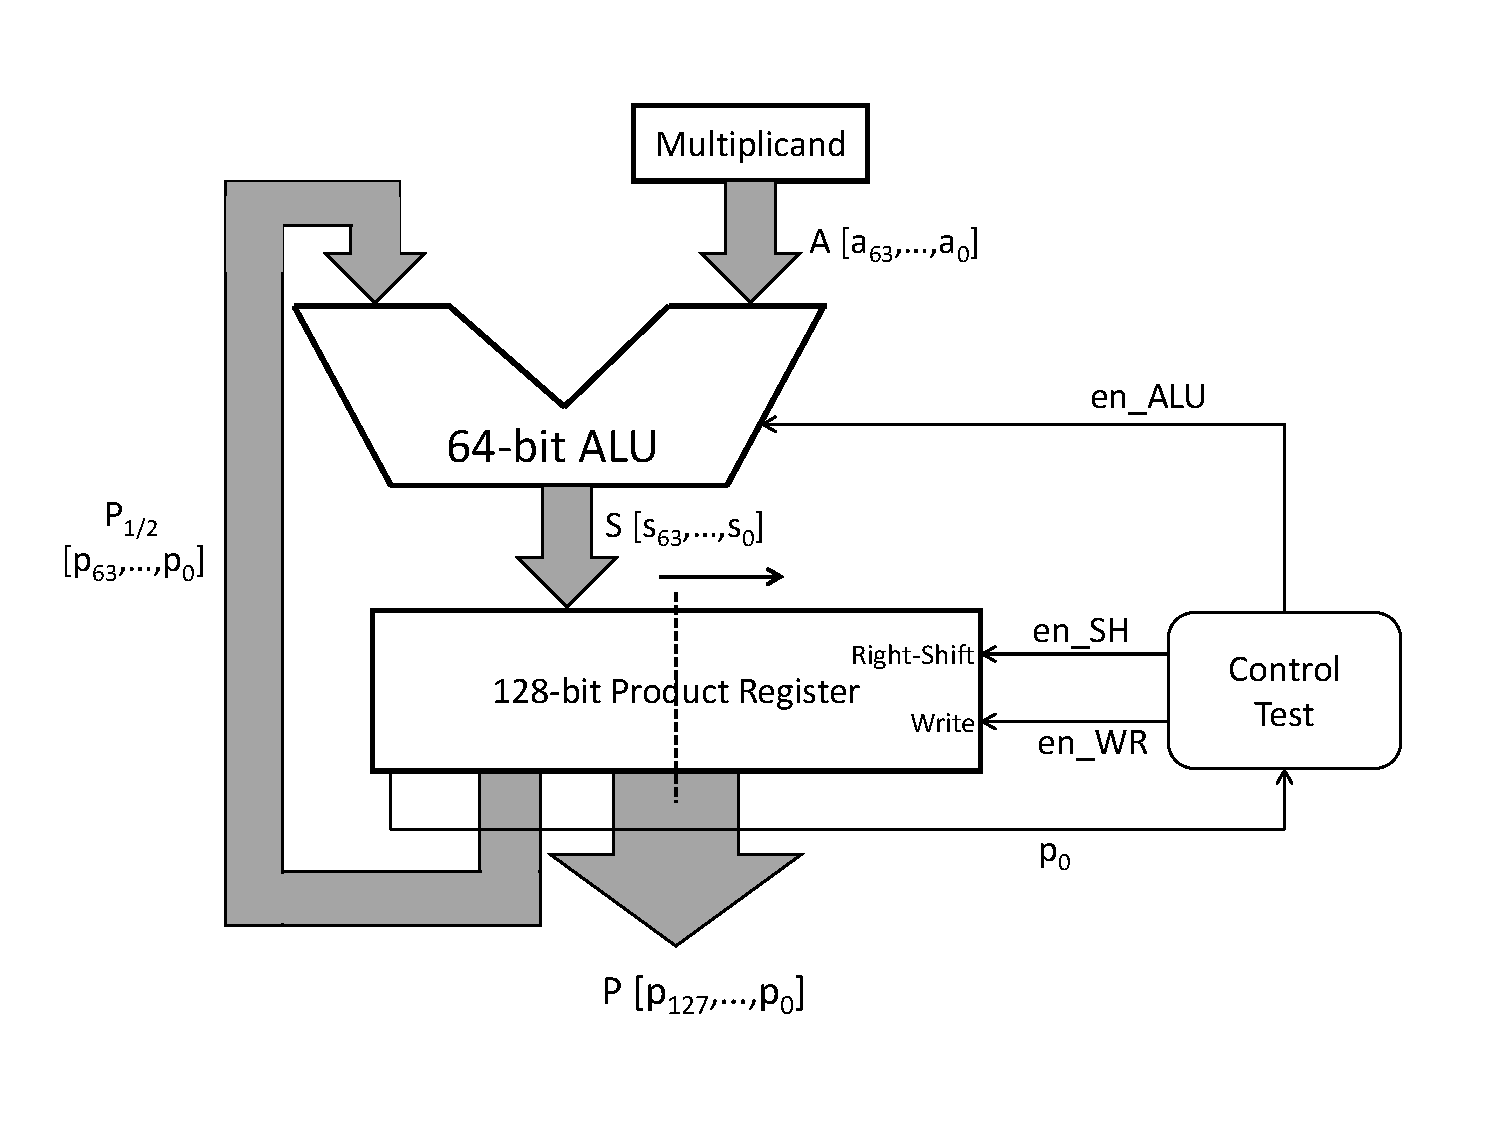
\includegraphics[width=\textwidth]{newfig/MIPS.pdf}
\caption{A 64-bit sequential multiplication hardware design}
\label{fig:MIPS}}
\end{figure}

Figure \ref{fig:MIPS} depicts a sequential multiplication hardware implementation within a 64-bit 
MIPS. Initially, one multiplicand is preloaded to the lower 64 bits of the product registers. 
Iteratively, the last significant bit (LSB) of current (temporary) product is used as flag to activate the ALU 
to add on the other multiplicand. For each iteration the data in product registers shifts right by 1 bit.
Finally when the most significant bit (MSB) of preloaded multiplicand arrives at the MSB of product registers,
the registers contains the result -- 128 bits product. The behavior can be described by the following algorithm:

% \vspace{0.2in}

\IncMargin{1em}
\begin{algorithm}[H]
\SetAlgoNoLine
\LinesNumbered
\Indm
 \KwIn{Multiplicand $A,B$}
 \KwOut{Product $C$}
\Indp

  Preload $B$ into lower 64-bit of Product Register $P$\;
  \Repeat{64 Repetitions}
  {
  	\If{Last Bit of Product Register $LSB(P)==1$}
  	{
		$P = P_{1/2}+B$\;
	}
	Right shift $P$\;
  }
\Return{$C=P$}
\caption {Sequential multiplication hardware in 64-bit MIPS}\label{alg:MIPS}
\end{algorithm}
\DecMargin{1em}

\vspace{0.2in}

% List the detailed bit-level property need to check P==P+B
Traditionally, to verify the functional correctness of this multiplier, satisfiability (SAT) based or BDD based 
model checking is applied on basic function units. For example, as a part of functional verification, 
we would like to check ``$P=P_{1/2}+B$" is correctly executed. Then in a model checker we need to add following 
specifications:

\begin{align*}
& en\_ALU \\
\land & s_0 = a_0 \oplus p_0 \\
\land & s_1 = a_1 \oplus p_1 \oplus (a_0 \land p_0) \\
\land & s_2 = a_2 \oplus p_2 \oplus ((a_1 \oplus p_1) \land a_0 \land p_0 \lor a_0 \land p_0) \\
\land & \cdots \\
\land & s_{63} = a_{63} \oplus p_{63} \oplus (c_{63})
\end{align*}

We can see that when checking a single part of the whole structure, the number of clauses 
needed will increase to $k+1$ when using $k$-bit datapath. Considering the formula representing 
carry-in will become longer and longer, the final conjunction of all clauses will contain 
$O(2^k)$ Boolean operators. If by some means we can write the specification with only 3 variables:
\begin{equation}
\label{eqn:wordspec}
S=P_{1/2}+B
\end{equation}

The abstraction to word-level will reduce symbolic storage and execution cost; the complexity 
to traverse the state space will be greatly reduced.
\end{Example}

On the other hand, when implementation details of the datapath are not available, it is not convenient 
any more for users of conventional model checker. The reason is that the user has to write all clauses 
for the implementation, which contains cross-literals, {\it e.g.} $s_2$ may associate with $a_1, p_0$, {\it etc.} If the user 
is not familiar with the implementation of this adder, those cross-literals will bring
confusions. However, if word-level techniques allow specification like Equation \ref{eqn:wordspec},
the verification tool will be very user-friendly and straightforward even if the implementation details
are in a black box.

\subsection{On the Existence of Word-Level Abstraction for Arbitrary Circuits}
When given a bit-level netlist, the prerequisites to use word-level techniques are to convert bit-level 
to word-level first. This conversion is usually completed by abstraction techniques.

An old but universally effective abstraction method is {\it Lagrange's interpolation}, 
which can be applied over finite fields. Here we use an example to illustrate the 
conversion in Galois field using Lagrange's interpolation for an arbitrary circuit.

\begin{Example}[Lagrange's interpolation]

\begin{figure}[H]
\centering{
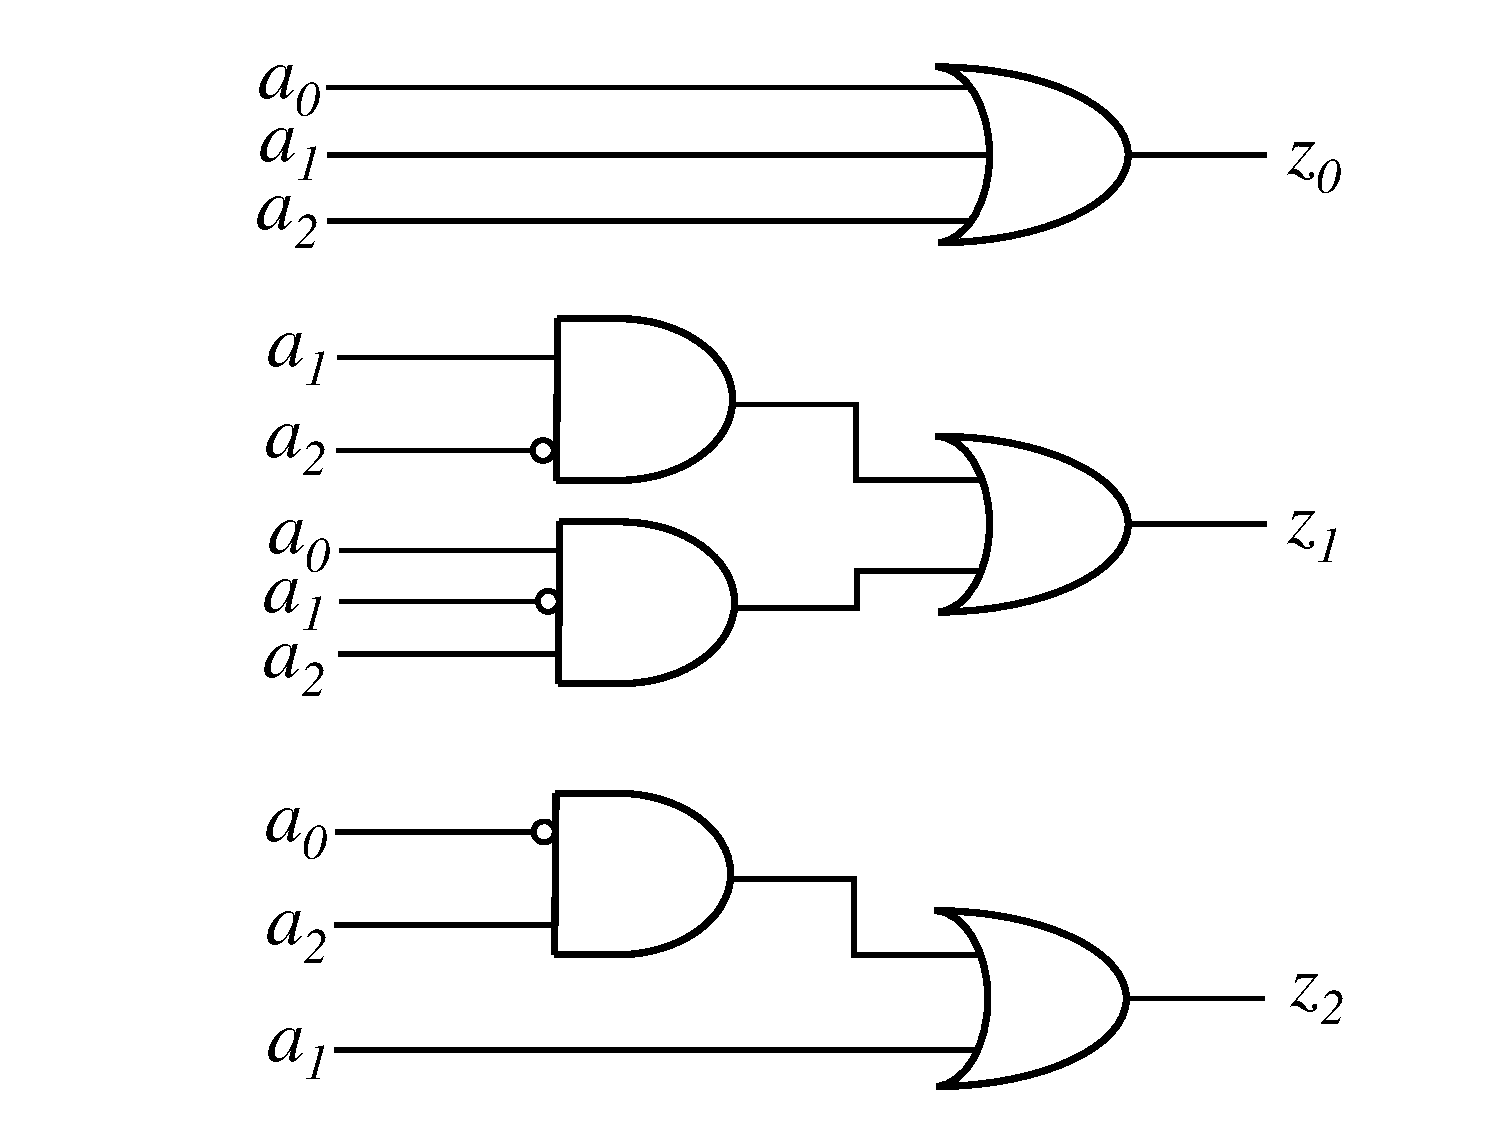
\includegraphics[width=4in]{newfig/Lagrange.pdf}
\caption{Gate-level netlist for Lagrange's interpolation example}
\label{fig:Lagrange}}
\end{figure}

Assume we are given gate-level netlist shown in Figure \ref{fig:Lagrange}. It can be written as 3 
Boolean equations:
\begin{align*}
z_0 &= a_0 \lor a_1 \lor a_2 \\
z_1 &= a_1 \land \neg a_2 \lor a_0 \land \neg a_1 \land a_2 \\
z_2 &= a_1 \lor \neg a_0 \land a_2
\end{align*}
Define 2 word-level variables $A,Z$ as input and output:
$$A = \{a_2a_1a_0\},~Z = \{z_2z_1z_0\}$$
To convert bit-level to word-level, we need to find mapping $\mathbb{B}^3 \rightarrow \mathbb{B}^3$,
or $\F_{2^3} \rightarrow \F_{2^3}$. The latter one, as mentioned in preliminaries, is a polynomial
function in $\F_{2^3}$.

For each element in $\F_{2^3}$, we write down the truth table as follows:
\begin{table}[H]
\label{tab:truthtable}
\centering{\small
\begin{tabular}{|c|ccc|c|}
\hline
$\{a_2a_1a_0\}\in\mathbb{B}^3$   & $A\in \F_{2^3}$ &$\rightarrow$& $\{z_2z_1z_0\}\in\mathbb{B}^3$  & $Z\in \F_{2^3}$ \\
\hline
000  &0 &$\rightarrow$&000 & 0 \\
001  &1 &$\rightarrow$&001 & 1 \\
010  &$\alpha$ & $\rightarrow$ & 111& $\alpha^2 + \alpha + 1$ \\
011  &$\alpha + 1$ &$\rightarrow$& 111 & $\alpha^2 + \alpha + 1$ \\
100  &$\alpha^2$ &$\rightarrow$& 101 &  $\alpha^2+1$ \\
101  &$\alpha^2 + 1$ &$\rightarrow$&011 & $\alpha+1$ \\
110  &$\alpha^2 + \alpha$&$\rightarrow$& 101 &$\alpha^2 + 1$ \\
111  &$\alpha^2 + \alpha + 1$ &$\rightarrow$& 101 &$\alpha^2 + 1$\\
\hline
\end {tabular}
}
\caption{Truth table for mappings in $\mathbb{B}^3$ and $\F_{2^3}$}
\end{table}
Now our objective is to abstract a function over finite field $\F_{2^3}$ in word-level variables, {\it i.e.} 
$Z = \Func(A)$. Recall Lagrange's interpolation formula:
\begin{equation}
\label{eqn:Lagrange}
\Func(x) =  \sum_{k=1}^N \left[ \prod_{(0\leq j \leq k-1),(j\neq i)}\frac{x-x_j}{x_i-x_j} \cdot y_k \right]
\end{equation}
The geometric meaning of Lagrange's interpolation in real algebra is: given $N$ points with coordinates $(x_i,y_i)$,
they can always be fitted into a polynomial function with at most $N-1$ degree, and that function can be 
written in the form of Equation \ref{eqn:Lagrange}. In this example, although defined in a Galois field instead of 
the real number field, the essential concept of Lagrange's interpolation remains the same. 
We can get 8 points in the affine space:
\begin{align*}
\text{Generic form}&: (a_2\alpha^2+a_1\alpha+a_0,z_2\alpha^2+z_1\alpha+z_0) \gets (A,Z) \\
\text{Point }1&: (0, 0) \gets (000,000) \\
\text{Point }2&: (1,1) \gets (001,001) \\
\text{Point }3&:  (\alpha,\alpha^2 + \alpha + 1) \gets (010,111)\\
\text{Point }4&:  (\alpha + 1,\alpha^2 + \alpha + 1)\gets (011,111) \\
\text{Point }5&:  (\alpha^2,\alpha^2+1) \gets (100,101)\\
\text{Point }6&:  (\alpha^2 + 1,\alpha+1)\gets (101,011)\\
\text{Point }7&:  (\alpha^2 + \alpha,\alpha^2 + 1)\gets (110,101)\\
\text{Point }8&:  (\alpha^2 + \alpha + 1,\alpha^2 + 1)\gets (111,101)
\end{align*}
Substitute 8 $(x_i,y_i)$ pairs in Equation \ref{eqn:Lagrange} with these 8 points in $\F_{2^3}$.
The result is a polynomial function with degree no greater than 7:
\begin{align*}
Z =& \Func(A) \\
=& (\alpha^2+\alpha+1) A^7 + (\alpha^2+1) A^6 + \alpha A^5 + (\alpha+1) A^4 \\
&+ (\alpha^2+\alpha+1)A^3+ (\alpha^2+1)A
\end{align*}

\end{Example}

The Lagrange's interpolation theorem also proves the existence of a word-level abstraction for a bit-level netlist.
In practice, Lagrange's interpolation is not scalable. 
The reason is that it needs the entire function (state space), but usually we only have the circuit representation
of the FSM. Considering this fact, a symbolic method is needed.
Our approach in this section uses abstraction based on 
Gr\"obner basis with abstraction term order (ATO), which is briefly introduced in Section \ref{sec:abstraction}.

\subsection{Significance of Developing Word-Level Reachability Analysis}
% At the end of this section, we summarize each subsection and conclude the motivation of our research.
% First, we start from the basic FSM traversal algorithms and exhibit their
% difficulties to overcome. Secondly, we state the observation that word-level description is 
% increasingly important and common in characterizing the data flow on modern large-size datapaths. 
% Last but not least, we give instances that some prerequisites for supporting word-level techniques 
% are already available. 

Based on the aforementioned discussions, the importance of performing FSM traversal at word-level 
can bring a dimension of abstraction in sequential circuit reachability analysis.
To overcome the cost incurred by searching in a large space, we propose to use word-level 
polynomials to represent the states and transition relations. As a result, states are categorized into 
sets represented by a small number of word-level polynomials (more specifically, the varieties to the polynomial ideals),
and multiple transition relations are therefore merged together. All of these efforts reduce the cost of 
state space, meanwhile lowering the time complexity to traverse such a state space. As Lagrange's interpolation
confirms the existence of word-level abstraction for bit-level circuits, the concept
can be extended to encode the state space of sequential circuit by word-level polynomials in $\Fkk$.
% we prove the feasibility of word-level techniques on general circuits' verification.
% Thus we cover both the necessity and sufficiency of developing such 
% a word-level traversal technique in our work.
% They are also answers to the questions at the beginning of this section.

\section{FSM Reachability using Algebraic Geometry}
\label{sec:reach}
% \subsection{An example illustrating our proposed approach}
We use symbolic state reachability with algebraic
geometry concepts. It is an abstraction based on word operand
definition of datapaths in circuits, and it can be applied
to arbitrary FSMs by bundling a set of bit-level variables together as
one or several word-level variables.  The abstraction polynomial,
encoding the reachable state space of the FSM, is obtained through
computing a GB over $\Fkk$ of the polynomials of the circuit using an
elimination term order based on Theorem \ref{thm:elimth}.  

\subsection{FSM Model for Sequential Circuits}
A finite state machine (FSM) is a mathematical model of computation for designing and analyzing sequential logic 
circuits. If a FSM's primary outputs depend on primary inputs and present state inputs, it is named as a \textit{Mealy machine};
the formal definition is as follows:
\begin{Definition}
A Mealy machine is an $n$-tuple $\mathcal M = (\Sigma,O,S,S^0,\Delta,\Lambda)$ where
\begin{itemize}
\item $\Sigma$ is the input label, $O$ is the output label;
\item $S$ is the set of states, $S^0\subseteq S$ is the set of initial states;
\item $\Delta:\ S\times\Sigma\to S$ is the next state transition function;
\item $\Lambda:\ S\times\Sigma\to O$ is the output function.
\end{itemize}
\end{Definition}
The other kind of FSM is \textit{Moore machine}, its difference from Mealy machine is that
its primary outputs only depend on the present states, {\it i.e.} the output function is defined as
$$\Lambda:\ S \to O$$
Typical sequential circuits can be depicted as Figure \ref{fig:seqmodel}(a). Primary inputs
$x_1,\dots,x_m \in \Sigma$, and primary outputs $z_1,\dots,z_n\in O$. Signals $s_1,\dots,s_k$ 
are present state (PS) variables, $t_1,\dots,t_k$ are next state (NS) variables.
We can define 2 $k$-bit words denoting the PS/NS variables as there are $k$ flip-flops
in the datapath: $S = (s_1,\dots,s_k), ~T=(t_1,\dots,t_k)$. Transition function
at bit level are defined as $\Delta_i$: 
$$t_i = \Delta_i(s_1,\dots,s_k,x_1,\dots,x_m)$$
\begin{figure}[H]
\centering{
%\begin{minipage}{12cm}
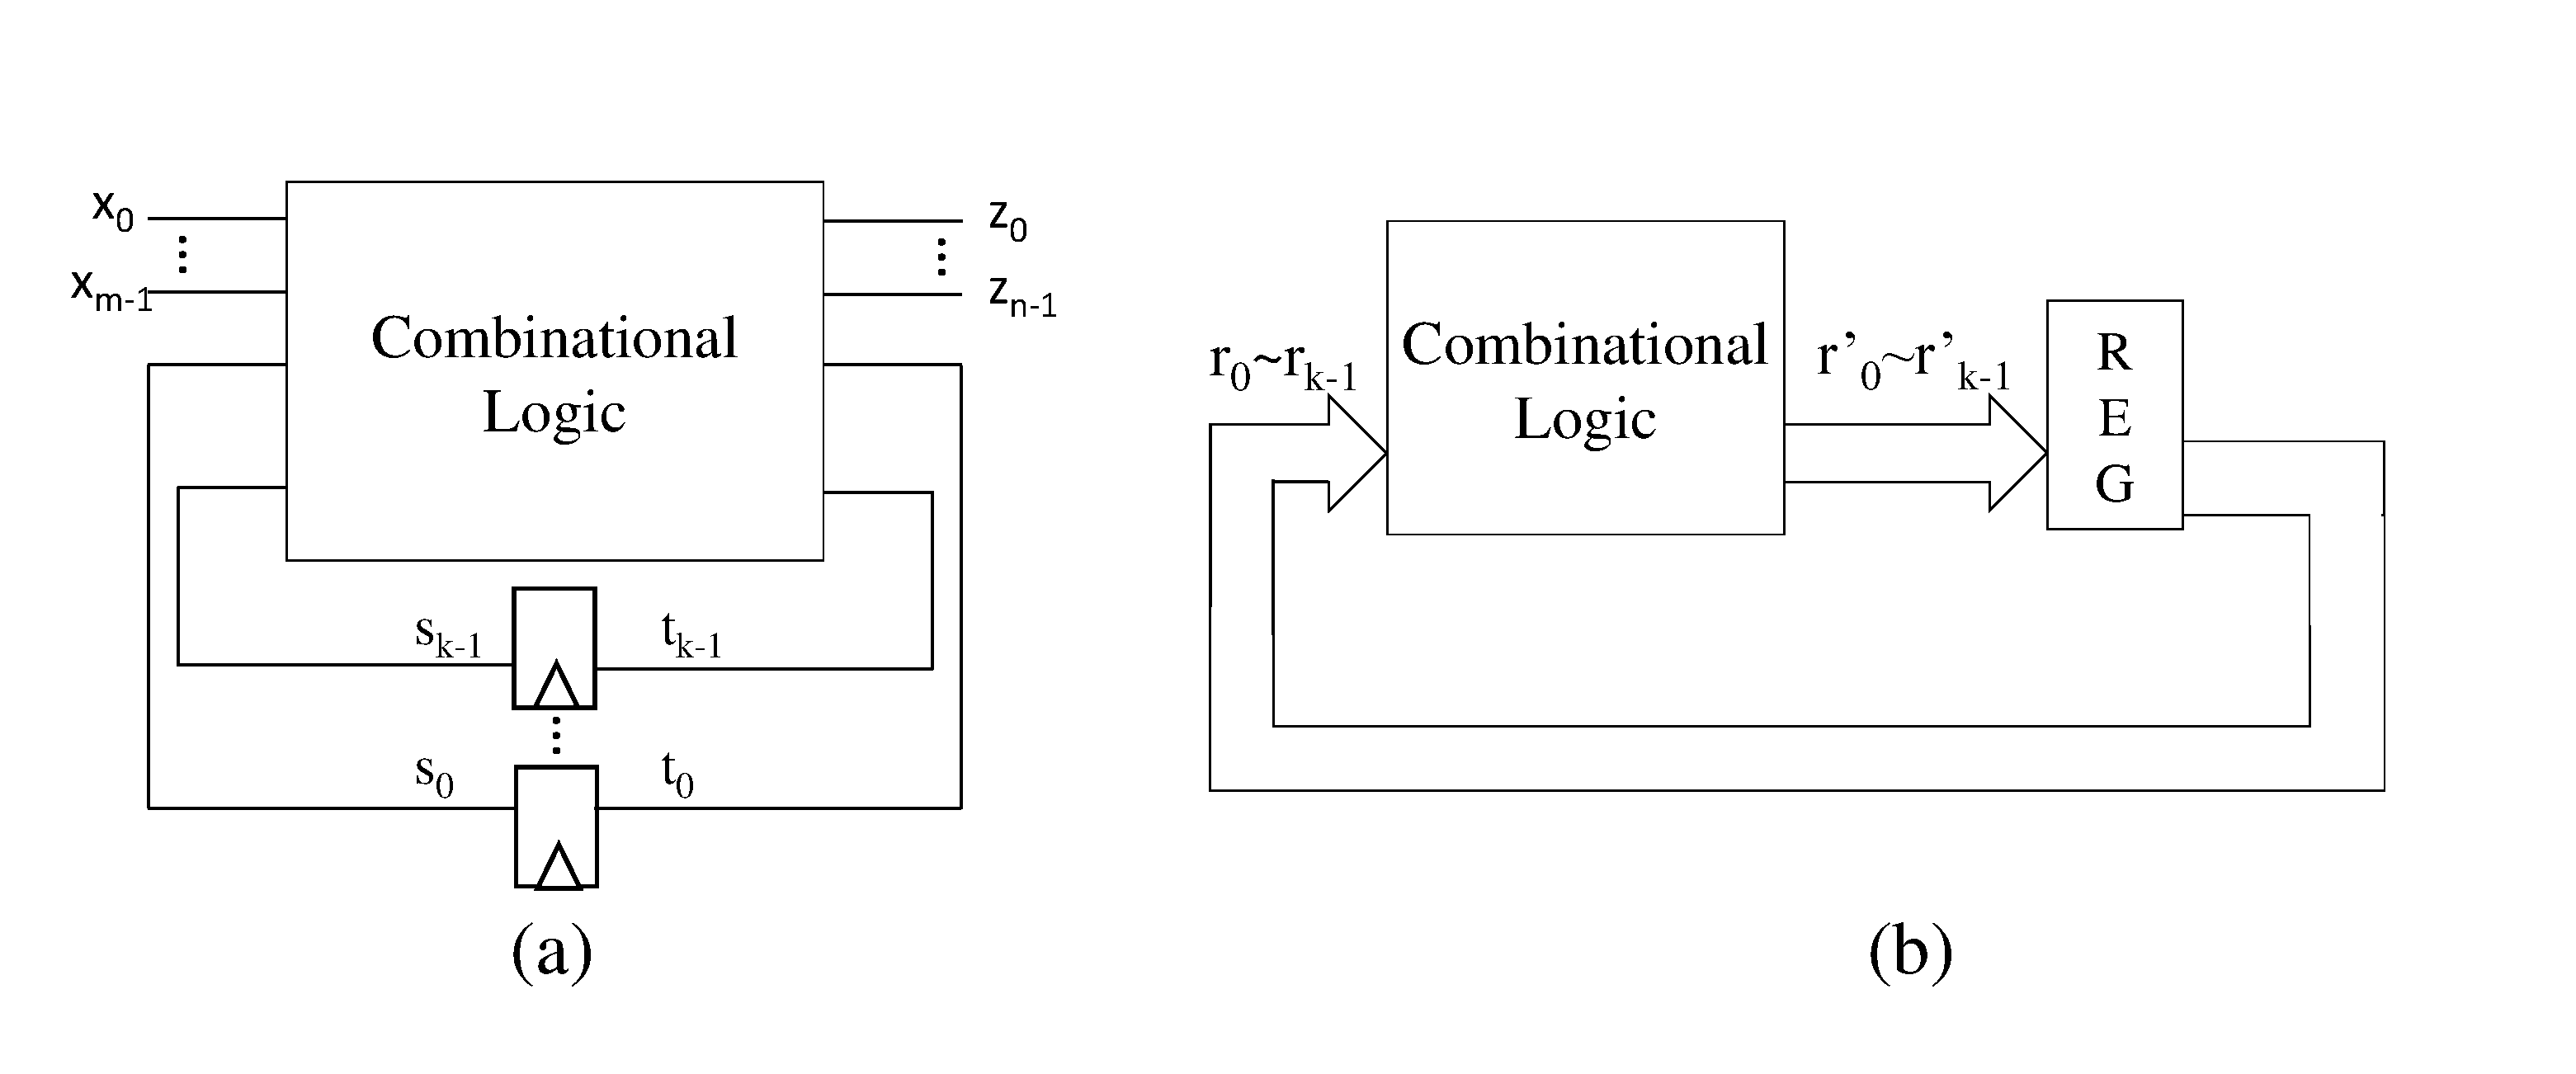
\includegraphics[width=5.5in]{newfig/seqmodel.pdf}
% \vspace{-0.2in}
\caption{FSM models of sequential circuits}
%\end{minipage}
\label{fig:seqmodel}}
\end{figure}
In some cases, arithmetic computations are implemented as Moore machines where input operands
are loaded into register files $R$ and the FSM is executed for $k$ clock cycles.
We can simplify them to the model in Figure \ref{fig:seqmodel}(b).

\subsection{Conventional Traversal Method}
Conceptually, the state-space of a FSM is traversed in a breadth-first
manner, as shown in Algorithm \ref{alg:BFS}. % \cite{KallaPartialScan}: 
The algorithm operates on the FSM $\mathcal{M} = (\sum, O, S, S^0,
\Delta, \Lambda)$ underlying a sequential circuit. In such cases, the
transition function $\Delta$ and the initial states are represented
and manipulated using Boolean representations such as BDDs or SAT
solvers. The variables $from, reached, to, new$ represent
characteristic functions of sets of states. Starting from the initial
state $from^i = S^0$, the algorithm computes the states reachable in
1-step from $from^i$ in each iteration. In line 4 of Algorithm
\ref{alg:BFS}, the {\it image computation} is 
used to compute the reachable states in every execution step. 

The {\it transition function} $\Delta$ is given by Boolean equations
  of the flip-flops of the circuit: $t_i = \Delta_i(s, x)$, where
  $t_i$ is a next state variable, $s$ represents the present   state
  variables and $x$ represents the input variables. The {\it
    transition relation of the FSM} is then represented as:  
\begin{equation} 
T(s, x, t) =   \prod_{i=1}^{n} (t_i \overline{\oplus } \Delta_i)
\end{equation}
where $n$ is the number of flip flops, and $\overline{\oplus}$ is XNOR
operation. Let $from$ denote the set of initial states, then the
image of the initial states, under the transition function $\Delta$ is
finally computed as:
\begin{align}
\label{eqn:img}
to = \text{Img}(\Delta, from) = \exists _s ~\exists _x ~[ T(s, x, t)
  \cdot from ] 
%= \exists _s ~\exists _x ~\prod_{i=1}^{n} (t_i \overline{\oplus } \Delta_i)\cdot from
\end{align}

Here, $\exists x (f)$ represents the {\it existential quantification
  of $f$ {\it w.r.t.} variable $x$}. In Boolean logic, this operator is implemented as
  $$\exists x (f) = f_x\lor f_{\overline{x}}$$





Let us describe the application of the algorithm on the  FSM circuit
of Figure \ref{fig:fsm}. {\it We will first describe its operation at the
Boolean level, and then describe how this algorithm can be implemented
using algebraic geometry at word level.} 

\begin{figure}[H]
\centering{
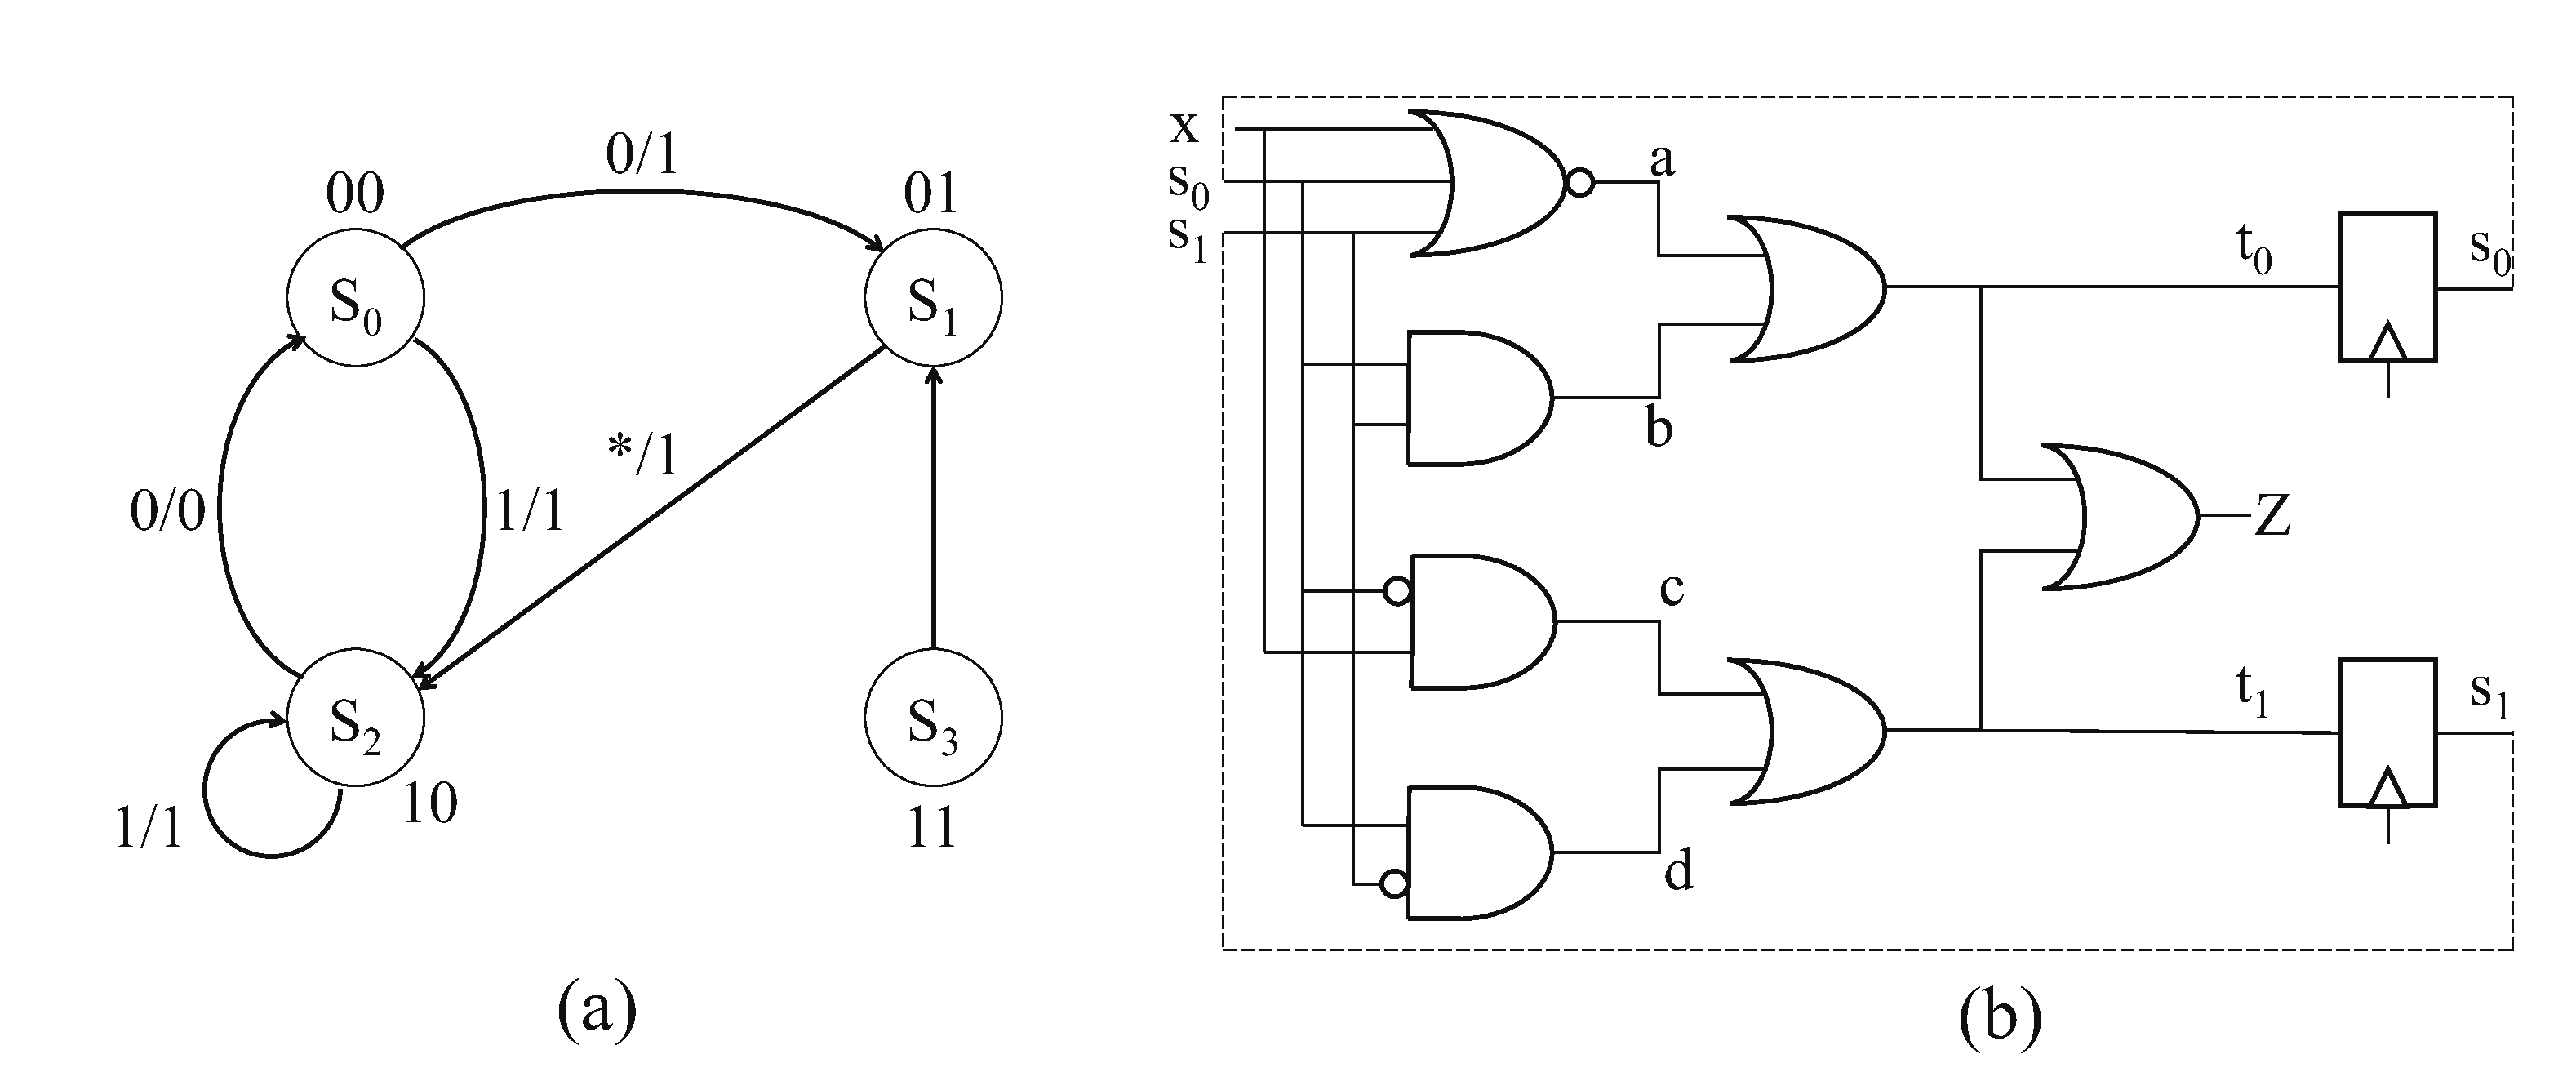
\includegraphics[width=\textwidth]{newfig/new_stg.eps}
\caption{The example FSM and the gate-level implementation. }
\label{fig:fsm}}
\end{figure}

In Line 1 of the BFS algorithm, assume that the initial state
is $S_3$ in Figure \ref{fig:fsm}(b), which is encoded as 
$S_3 = \{11\}$. Using Boolean variables $s_0, s_1$ for the present
states, $from^0 = s_0\cdot s_1$ is represented as a Boolean formula. 



\begin{Example}
For the circuit in Figure \ref{fig:fsm}(b), we have the transition
functions of the machine as:

\begin{align*}
\Delta_1: & ~t_0 \overline{\oplus} ((\overline{x \vee s_0 \vee s_1}) \vee s_0 s_1)\\
\Delta_2: & ~t_0 \overline{\oplus} (\overline{s_0}x \vee \overline{s_1}s_0)\\
from:     & ~from^0 = s_0\cdot s_1
\end{align*}

When the formula of Equation \ref{eqn:img} is applied to compute 1-step
reachability, $to = \exists _{s_0, s_1, x} (\Delta_1 \cdot \Delta_2
\cdot from^0)$, we obtain $to = \overline{t_0}\cdot t_1$, which denotes
the state $S_1 = \{01\}$ reached in 1-step from $S_3$.
In the next iteration, the algorithm uses state $S_1 = \{01\}$ as the
current (initial) state, and computes $S_2 = \{10\} = t_0\cdot
\overline{t_1}$ as the next reachable state, and so on. 
\end{Example}

%% Let  $\Delta_i$ denote the transition function for $i^{th}$ bit of the
%% output $T$
%% (denoted by $t_i$), and it is described by a Boolean function. We can
%% obtain the transition relation  for bit-vector $T$:
%% $Tran(s_0,s_1,x,t_0,t_1) =
%% \bigwedge_{i=1}^{2}(t_i\ \bar{\oplus}\ \Delta_i)$. Assume present
%% states are represent by Boolean formulas $PS(s_0,s_1)$, then the image
%% function is written as $\text{Img}(Tran,\ PS) =
%% \exists_{s_0,s_1}\exists_{x}[Tran(s_0,s_1,x,t_0,t_1)\land
%%   PS(s_0,s_1)]$, where $\exists_x f$ denotes the existential
%% quantification of $f$ w.r.t. $x$. 

Our objective is to model the transition functions $\Delta$ as a
polynomial ideal $J$, and to perform the image computations 
%(Algorithm \ref{alg:BFS}, line 4) 
using Gr\"obner bases over Galois fields. {\it
This requires to perform quantifier elimination; which can be
accomplished using the GB computation over $\Fkk$ using elimination
ideals} \cite{gao:qe-gf-gb}. Finally, the set union, intersection and
complement operations are also to be implemented in algebraic geometry.

\subsection{FSM Traversal at Word-Level over $\Fkk$} 
The state transition graph (STG) shown in Figure \ref{fig:fsm}(a) uses a
2-bit Boolean vector to represent 4 states $\{S_0, S_1, S_2,
S_3\}$. We map these states to elements in $\mathbb{F}_{2^2}$, where
$S_0 = 0, S_1 = 1, S_2 = \alpha, S_3 = \alpha+1$. Here, we take 
$P(X) = X^2+X+1$ as the irreducible polynomial to construct
$\mathbb{F}_4$, and $P(\alpha) = 0$ so that $\alpha^2 + \alpha + 1 =
0$.  

{\it Initial state:} Line 1 of Algorithm \ref{alg:BFS} specifies the initial state.
In algebraic geometry, it can be specified by means of a corresponding polynomial
 $f = \mathcal{F}(S) =
S - 1 - \alpha$. Notice that if we consider the ideal generated by the
initial state polynomial, $I = \langle f\rangle$, then its variety
$V(I) = 1+\alpha$ corresponds to the state encoding $S_3 = \{11\} =
1+\alpha$, where a polynomial in word-level variable $S$ encodes the
initial state. 
% with only one generator $f$, its variety
% $V(I) = \{\gamma\ |\ \gamma \in \mathbb{F}_{2^2}, \gamma = 1+\alpha\}$, which equals to $\{1+\alpha\}$, the only
% valid value $S_3$ can take.


%Using theorems from Section \ref{sec:elim}, we implement the image
%function by a GB computation on elimination ideal. Ex.\ref{ex:motiv}
%is an example for our implementation of image function, i.e. one-step
%reachability. 

{\bf Set operations:} In Lines 5 and 6 of
Algorithm  \ref{alg:BFS}, we need  \textbf{union}, 
\textbf{intersection} and \textbf{complement} of varieties over
$\mathbb{F}_{2^k}$, for which we again use algebraic geometry concepts.

\begin{Definition}
\label{def:sum}
({\bf Sum/Product of Ideals} \cite{ideals:book}) If $I = \langle f_1,
\dots, f_r\rangle$ and $J = \langle g_1, \dots, g_s\rangle$ are
ideals in $R$, then the {\bf sum} of $I$ and $J$ is defined as $I + J
= \langle f_1, \dots, f_r, g_1, \dots, g_s\rangle$. Similarly, the
{\bf product} of $I$ and $J$ is $I \cdot J = \langle
f_ig_j\ |\ 1 \leq i \leq r, 1 \leq j \leq s\rangle$. 
\end{Definition}

%With concepts of ideal sums and products, we can obtain the
%intersection and union of affine varieties as:
\begin{Theorem}
\label{thm:unionintersect}
If $I$ and $J$ are ideals in $R$, then 
${\bf V}(I + J) = {\bf V}(I) \bigcap {\bf V}(J)$ and ${\bf V}(I \cdot
J) = {\bf V}(I) \bigcup {\bf V}(J)$. 
\end{Theorem}


In Line 5 of Algorithm  \ref{alg:BFS}, we need to compute the complement of a
set of states. Assume that $J$ denotes a polynomial ideal whose
variety $V(J)$ denotes a set of states. We require the computation of
another polynomial ideal $J'$, such that $V(J')=\overline{V(J)}$. We
show that this computation can be performed using the concept of {\bf
  ideal quotient}:  

\begin{Definition}
\label{def:quo}
({\bf Quotient of Ideals}) If $I$ and $J$ are ideals in a ring $R$, then $I:J$ is the set
%  \begin{equation}
  $\{f \in R \ |\ f\cdot g \in I, \forall g \in J\}$ %\nonumber
%  \end{equation}
and is called the {\bf ideal quotient} of $I$ by $J$.
\end{Definition}

%The following example shows a simple ideal quotient operation:
\begin{Example}
In $\Fq[x,y,z]$, ideal $I = \langle xz,yz\rangle$, ideal $J = \langle z\rangle$. Then
\begin{align*}
I:J &= \{f\in\Fq[x,y,z]~|~f\cdot z \in \langle xz,yz\rangle\} \\
&= \{f\in\Fq[x,y,z]~|~f\cdot z = Axz+Byz\}\\
&= \{f\in\Fq[x,y,z]~|~f= Ax+By\}\\
&= \langle x,y\rangle
\end{align*}
\end{Example}

% However, complement of variety cannot be easily dealt by simple arithmetic on polynomial generators.
% For non-trivial cases we can only prove that 
% \begin{Theorem}
% Let $I, J$ be ideals in $\mathbb F[x_1,\dots,x_n]$, then 
% $${\bf V}(I:J) \supset {\bf V}({\bf I}({\bf V}(I) - {\bf V}(J)))$$
% \end{Theorem}
% Fortunately for most hardware verification cases, the form of polynomial generators are restricted.
% A proposition has been proved by \cite{jinpeng} that after adding {\bf vanishing polynomials ideal}
% the new composed ideal implies following corollary:

We can now obtain the complement of a variety through the following
results which are stated and proved below:

\begin{Lemma}
\label{lem:gcd}
Let $f,g\in \Fkk[x]$, then $\langle f:g\rangle = \left\langle\frac{f}{gcd(f,g)}\right\rangle$.
\end{Lemma}

\begin{Proof}
Let $d = gcd(f, g)$. So, $f = df_1 , g = dg_1$ with $gcd(f_1 , g_1 ) =
1$. Note that $f_1 = \frac{f}{gcd(f,g)}$.

Take $h \in \langle f : g\rangle$. According to the
Definition \ref{def:quo}, $hg \in \langle f \rangle$, which means $hg = f
\cdot r$ with $r \in \Fkk[x]$. Therefore, $hdg_1 = df_1 r$ and $hg_1 =
f_1 r$. But considering $gcd(g_1 , f_1 ) = 1$ we have the fact that
$f_1$ divides $h$. Hence $h \in \langle f_1\rangle$.

Conversely, let $h \in \langle f_1 \rangle$. Then $h = s \cdot f_1$,
where $s \in \Fkk[x]$. So, $hg = hdg_1 = sf_1 dg_1 = sg_1 f \in 
\langle f \rangle$. Therefore, $h \in \langle f : g\rangle$.
\end{Proof}


\begin{Theorem}
\label{thm:quotient}
Let $J$ be an ideal generated by a single univariate polynomial in
variable $x$ over $\Fkk[x]$, and let the vanishing ideal $J_0 = \langle
x^{2^k}-x\rangle$. Then  
$${ V}(J_0:J) = { V}(J_0) - { V}(J),$$ where all the varieties are
considered over the field $\Fkk$. 
\end{Theorem}

\begin{Proof}
Since $\Fkk[x]$ is a principal ideal domain, $ J = \langle g(x)\rangle$
for some polynomial $ g(x) \in \Fkk[x]$. Let $h(x) = gcd(g(x), x^{2^k} -
x)$. So, $g(x) = h(x)g_1(x) , x^{2^k} - x = h(x)f_1(x)$, with $gcd(f_1(x) , g_1(x) ) =
1$. Then $J_0 : J = \langle f_1(x) \rangle$ by Lemma \ref{lem:gcd}. 

Let $x \in V(J_0 ) - V(J)$. From the definition of set
complement, we get $x \in \Fkk$ while $g(x) \neq 0$.  

Since $x^{2^k} = x$, we see that either $h(x) = 0$ or $f_1 (x) =
0$. Considering $g(x) \neq 0$, we can assert that $h(x) \neq 0$. In
conclusion, $f_1 (x) = 0$ and $x \in V(f_1 )$. 

Now let $x \in V(f_1 )$, we get $f_1 (x) = 0$. So, $x^{2^k} - x = 0$
gives $x \in V(J_0) = \Fkk$ which  contains all elements in the
field. 

Now we make an assumption that $x \in V(g)$. Then $g(x) = 0 =
d(x)g_1(x)$ which means either $h(x) = 0$ or $g_1 (x) = 0$. 

If $g_1 (x) = 0$, then since $f_1 (x) = 0$ we get that $f_1(x) , g_1(x)$
share a root. This contradicts the fact that $gcd(f_1(x) , g_1(x) ) = 1$.

On the other hand, if $h(x) = 0$, then since $f_1 (x) = 0$ and
$x^{2^k} - x = d(x)f_1(x)$, we get that $x^{2^k} - x$ has a double root. 
But this is impossible since the derivative of $x^{2^k} - x$ is $-1$.

So, $x \notin V(g(x))$ and this concludes the proof.
\end{Proof}

% Let $J_0 = \langle x_1^{2^k} - x_1, \dots, x_n^{2^k} - x_n \rangle$
% denote the ideal of all vanishing polynomials in $\Fkk$. Then, we have
% $V(J_0) = (\Fkk)^{n}$; i.e. the variety of vanishing ideal contains
% all possible valuations of variables, so it constitutes the {\bf
%   universal set}. Subsequently, based on Theorem \ref{thm:quotient},
% the {\bf absolute complement} $V(J')$ of a variety $V(J)$ can be
% computed as: 

Let $x^{2^k}-x$ be a vanishing polynomial in $\Fkk[x]$. Then $V(x^{2^k}-x)=\Fkk$
{\it i.e.} the variety of vanishing ideal contains
 all possible valuations of variables, so it constitutes the {\bf
   universal set}. Subsequently, based on Theorem \ref{thm:quotient},
 the {\bf absolute complement} $V(J')$ of a variety $V(J)$ can be
 computed as: 

\begin{Corollary} \label{cor:complement}
Let $J\subseteq \Fkk[x]$ be an ideal, and $J_0=\langle x^{2^k}-x\rangle$. Let $J'$ be an ideal 
computed as $J' = J_0:J$. Then $$V(J') = \overline{V(J)} = {V}(J_0:J)$$
\end{Corollary}

With Corollary \ref{cor:complement}, we are ready to demonstrate the
concept of word-level FSM traversal over $\Fkk$ using algebraic
geometry. The algorithm is given in Algorithm \ref{alg:univa}. Note that in
the algorithm, $from^i, to^i, new^i$ are {\it univariate polynomials in variables $S$
or $T$} only, due to the fact that they are the result of a GB
computation with an elimination term order, where the bit-level 
variables are abstracted and quantified away.

\section{Problem Setup and Formulation}
\begin{Problem}
We use the notions from Figure \ref{fig:seqmodel}(a) in this setup. 
\begin{enumerate}[{1)}] 
\item The circuit is modeled over $\Fkk = \F_2[x]\pmod{p(x)}, p(\alpha) = 0$, where $k$ is the number of flip-flops,
	the PS variables $\{s_0,\dots,s_{k-1}\}$, NS variables $\{t_0,\dots,t_{k-1}\}$.
\item Denote $S$ as the PS word-level by the following polynomial:
$$f_S: S = s_0+s_1\alpha+s_2\alpha^2+\cdots+s_{k-1}\alpha^{k-1}$$
Similarly we define NS word-level variable $T$ by:
$$f_T: T = t_0+t_1\alpha+t_2\alpha^2+\cdots+t_{k-1}\alpha^{k-1}$$
\item Impose ATO for sequential circuits which is 
$$LEX: \text{ all bit-level variables in any order }>S>T$$
\item Write polynomials $f_1,\dots,f_s$ for each gate, and construct ideal describing the circuit:
$$J_{ckt} = \langle f_1,\dots,f_s,f_S,f_T\rangle$$
as well as the ideal with vanishing polynomials:
$$J_0 = \langle \dots,x_i^2-x_i,\dots,S^{2^k}-S,T^{2^k}-T\rangle$$
where $x_i$ corresponds to bit-level variables denoting wires in the circuit.
\item Compute GB with ATO for $G$. Then obtain the projection of variety only on NS variable $T$, by
$$G\cap \Fkk[T]$$
\end{enumerate}
\end{Problem}


\IncMargin{1em}
\begin{algorithm}[hbt]
\SetAlgoNoLine
\LinesNumbered
\Indm
 \KwIn{The circuit's characteristic polynomial ideal $J_{ckt}$,
   initial state polynomial $\F(S)$, and LEX term order: bit-level
   variables $x, s, t$ $>$ PS word $S$ $>$ NS word $T$}
\Indp

  $from^0 = reached = \Func(S)$\;
  \Repeat{$\langle new^i\rangle == \langle 1\rangle$}
  {
  	$i \gets i + 1$\;
  	$G \gets$GB($\langle J_{ckt},J_v, from^{i-1}\rangle$)\;
  	\tcc{Compute Gr\"obner basis with elimination term order: $T$ smallest}
	$to^i \gets G\cap \Fkk[T]$\;
	\tcc{There will be a univariate polynomial in $G$ denoting the
          set of next states in word-level variable $T$}
	$\langle new^i\rangle \gets \langle to^i\rangle + (\langle T^{2^k}-T\rangle:\langle reached\rangle)$\;
	\tcc{Use quotient of ideals to attain complement of reached states, then use sum of ideals to attain an intersection with next state}
  	$\langle reached\rangle \gets \langle reached\rangle \cdot \langle new^i\rangle$\;
  	\tcc{Use product of ideals to attain a union of newly reached states and formerly reached states}
	$from^i \gets new^i(S\setminus T)$\;
	\tcc{Start a new iteration by replacing variable $T$ in newly reached states with current state variable $S$}
  }
  \tcc{Loop until a fixpoint reached: newly reached state is empty}
\Return{$\langle reached\rangle$}
\caption {Algebraic Geometry based FSM Traversal}\label{alg:univa}
\end{algorithm}
\DecMargin{1em}

\subsection{Word-Level FSM Traversal Example}
\begin{Example}
\label{ex:SMPO}
We apply Algorithm \ref{alg:univa} to the example shown in
Figure \ref{fig:fsm} to execute the FSM traversal. Let the initial state
$from^0 = \{00\}$ in $\B^2$ or $0 \in \mathbb F_4$. Polynomially, it is
written as $from^0 = S - 0$. In the first iteration, we compose
an ideal $J$ with 

%\begin{minipage}[h]{0.4\textwidth}
\begin{align*}
&f_1: t_0- (xs_0s_1+xs_0+xs_1+x+s_0+s_1+1)\\
&f_2: t_1 - (xs_0+x+s_0s_1+s_0)\\
&f_3: S - s_0 - s_1\alpha; ~~~f_4: T - t_0 - t_1\alpha
\end{align*}
$J_{ckt} = \langle f_1,f_2,f_3,f_4\rangle$, and the vanishing
polynomials: 
%\end{minipage}
%\begin{minipage}[h]{0.6\textwidth}

\begin{align*}
&f_5: x^2-x; ~~f_6: s_0^2-s_0, ~~f_7: s_1^2-s_1\\
&f_8: t_0^2-t_0, ~~f_9: t_1^2-t_1; ~~f_{10}: S^4-S, ~~f_{11}:T^4-T
\end{align*}
with $J_v = \langle f_5,f_6,\dots,f_{11}\rangle$.
%\end{minipage}

%and $from^0$. 

Compute $G = GB(J)$ for $J = J_{ckt}+J_0+\langle from^0\rangle$,
with an elimination term order 
$$ \underbrace{\{x,s_0,s_1,t_0,t_1\}}_{\text{all bit-level variables}} 
> \underbrace{S}_{\text{(PS~word)}} > \underbrace{T}_{\text{(NS~word)}}.$$

The resulting GB $G$ contains a polynomial generator with only $T$ as
the variable. In Line 5, assign it to the next state $$to^1 =
T^2+(\alpha+1)T+\alpha.$$ Note that the roots or variety of
$T^2+(\alpha+1)T+\alpha$ is $\{1, \alpha\}$, denoting the states
$\{01,10\}$. 

Since the formerly reached state ``$reached = T$'', its complement is
computed using Corollary \ref{cor:complement} 
$$\langle T^4-T\rangle:\langle T\rangle
= \langle T^3+1\rangle.$$ 

$V(\langle T^3 + 1\rangle) = \{1, \alpha, \alpha+1\}$ denoting the states
$\{01,10,11\}$. Then the newly reached state set in this iteration is 
$$\langle T^3+1, T^2+(\alpha+1)T+\alpha \rangle = \langle
T^2+(\alpha+1)T+\alpha \rangle$$ We add these states 
to formerly reached states 
\begin{align*}
reach &= \langle T\rangle \cdot \langle T^2+(\alpha+1)T+\alpha \rangle \\
&= \langle T\cdot T^2+(\alpha+1)T+\alpha \rangle \\
&= \langle T^3+(\alpha+1)T^2+\alpha T\rangle
\end{align*}
 {\it i.e.} states $\{00,01,10\}$. We update the present states
for next iteration $$from^1 = S^2+(\alpha+1)S+\alpha.$$ 

In the second iteration, we compute the reduced GB with the same term
order for ideal $J = J_{ckt}+J_v+\langle from^1\rangle$. 
It includes a polynomial generator $$to^2 = T^2+\alpha T$$ denotes states
$\{00,10\}$. The complement of $reached$ is $$\langle T^4-T\rangle:\langle T^3+(\alpha+1)T^2+\alpha T\rangle
= \langle T + 1+\alpha\rangle$$ ({\it i.e.} states $\{11\}$). We compute the newly reached state 
$$\langle T^2+\alpha T, T+1+\alpha \rangle = \langle 1\rangle$$ 

Since the GB contains the unit ideal, it means the newly reached state
set is empty, thus a fix-point has been reached. The algorithm
terminates and returns $$reached = \langle T^3+(\alpha+1)T^2+\alpha
T\rangle$$ which, as a Gr\"obner basis of the elimination ideal,
canonically encodes the final reachable state set. 
\end{Example}

% {\it Significance of using GB:} A reduced GB is a unique, minimal and
% {\it canonical} representation of the circuit's function. Starting
% from a certain initial state and using a reduced GB to represent the
% transition function, reachable states can be computed and represented
% canonically. Then it becomes possible to identify  when a fixpoint
% is reached (termination of the algorithm) by performing an equality
% check of polynomial ideals. Moreover, the GB computation is also used
% as a quantification procedure. As the GB is computed w.r.t. an
% elimination term order with ``bit-level variables'' $>$
% ``present-state word'' $S$ $>$ ``next-state word'' $T$, the set of
% reachable states are encoded, canonically, using a univariate
% polynomial in $T$, quantifying away the rest of the variables. 

\subsection{Significance of using Algebraic Geometry and Gr\"obner Bases}
The essence of our approach is based on algebraic geometry and Gr\"obner basis concepts.
One the one hand, we use GB with elimination term ordering as an analog of image function.
As mentioned in Section \ref{sec:abstraction}, we construct the ideal $J+J_0$ to 
describe the circuit in Figure \ref{fig:proj_reacha} using algebraic geometry.
Given the present states, the next states are implicitly represented in the variety of 
the elimination ideal obtained by quantify away the remaining variables. 
This projects the variety on the NS output $T$ by eliminating all other variables.
This projection gives us the canonical representation of NS in a polynomial in $T$.

\begin{figure}[H]
\centering{
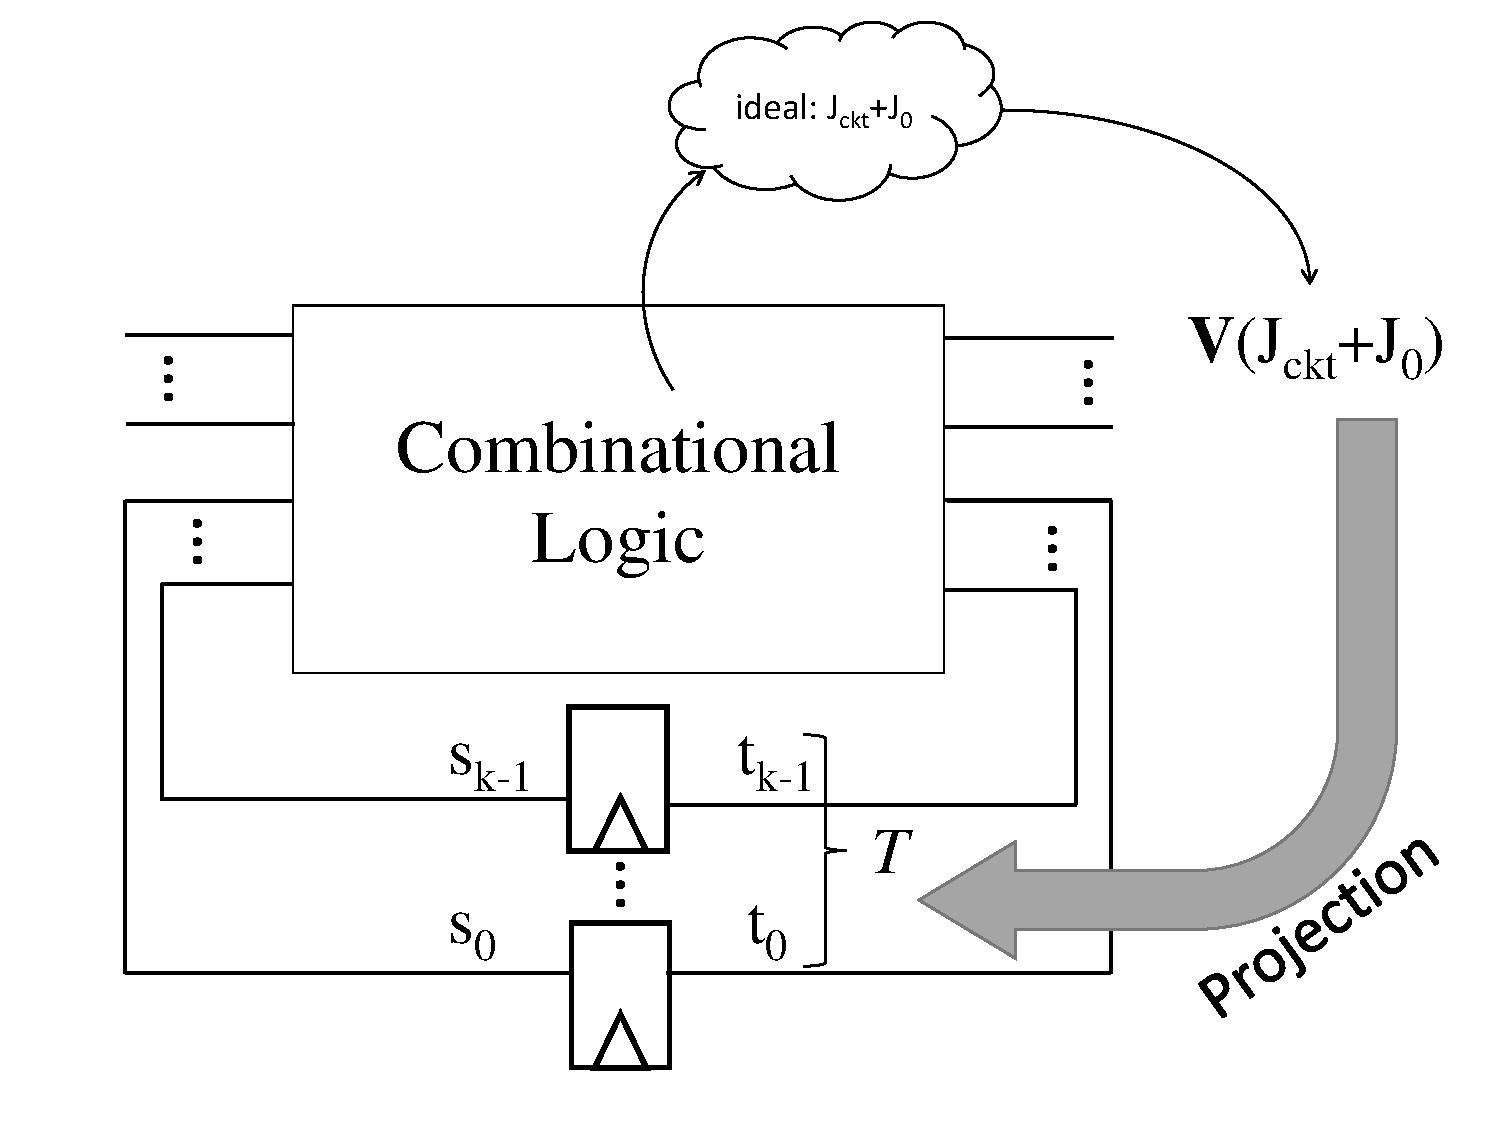
\includegraphics[width=\textwidth]{newfig/proj_reacha.pdf}
\caption{Projection of the variety of circuit description ideal}
\label{fig:proj_reacha}}
\end{figure}

On the other hand, we use the algebraic ideals to implement set operations. States are finite set of points,
which can be mapped to a variety.
In algebraic geometry, manipulating the ideals provides a mechanism to 
operate on the varieties without actually solving the system of equations. The intersection, union and 
complement of varieties are mapped to varieties of the sum, product and quotient of ideals, respectively.
% Furthermore, the varieties are equivalent to set of states because of correspondence of 
% affine space and state space.

As a result, we create the analog of the FSM traversal algorithm in algebraic geometry which is 
compatible with word-level variables ({\it e.g.} $S,T$). We show it is effective to perform the 
reachability analysis.

\section{Improving our Approach}
\label{sec:improve}

Using elimination term ordering on computing GB for large set of polynomial is time-consuming, and usually 
intractable. The reason is the exponential computational complexity \cite{gao:gf-gb-ms}:
\begin{Theorem}
Let $J+J_0 = \langle f_1, \dots, f_s, ~x_1^q - x_1, \dots, x_d^q -
x_d\rangle \subset \Fq [x_1, \dots, x_d]$ be an ideal. The time and
space complexity of Buchberger's algorithm to compute a \Grobner
basis of $J+J_0$ is bounded by $q^{O(d)}$.
\end{Theorem}

In our case $q = 2^k$, and when $k$ and $d$ are large, this complexity 
makes abstraction infeasible.

Buchberger's algorithm consists of two major operations: one is finding 
$Spoly$ pairs, the other is dividing the $Spoly$ by the set of polynomials.
Its actual cost is very sensitive to the term ordering: if there exists 
a term order making most $Spoly$ computation unnecessary, then the cost to 
compute $Spoly$ is saved. Moreover, it prevents the generation of new polynomials 
from unnecessary $Spoly$ reductions, which further reduces the cost
because there are less $Spoly$ pairs as well as candidate divisors.
Besides tuning the term ordering, directly cutting down the number of 
polynomials in the set is also effective.

In order to make our approach scalable, we propose improvements from 
two aspects: 1) using another term ordering which can lower the 
computational complexity of obtaining GB; and 2) reducing the number of
polynomials by collecting bit-level primary inputs (PIs) and integrating them as word-level 
variables which are compatible with our working GF.

\subsection{Simplifying the Gr\"obner Bases Computation}
In Algorithm \ref{alg:univa}, a Gr\"obner basis is computed for each
iteration to attain the word-level polynomial representation of the next states. In practice, for 
a sequential circuit with complicated structure and large size, Gr\"obner basis computation
is intractable. To overcome the high computational complexity of computing a GB, 
we describe a method that computes a GB of a smaller subset of polynomials.
The approach draws inspirations from \cite{pruss:tcad15}, which defined and justified a 
{\it refined abstraction term order} (RATO). The following definition rephrases Definition 5.1 in \cite{pruss:tcad15}
with our sequential circuit setup and notations.

% From Tim's journal
\begin{Definition}[Refined Abstraction Term Order $>_r$]
Starting from the pseudo outputs (NS variables) of the combinational component of a sequential circuit $C$, 
perform a reverse topological 
traversal toward the pseudo inputs (PS variables) and primary inputs. Order each variable of the circuit according to
its reverse topological order. Impose a LEX term order $>_r$ on $\Fq[x_1,\dots,x_d,T,S]$
with the ``bit-level variables $x_1,\dots,x_d$ ordered reverse topologically "$ > T>S$,
this term order is called RATO.
\end{Definition}


According to proposition 5.1 in \cite{pruss:tcad15}, if the GB is computed using RATO, 
there will be only one pair of polynomials $\{f_w,f_g\}$ such that 
their leading monomials are not relatively prime, {\it i.e.} 
$$gcd(LM(f_w), LM(f_g)) \neq 1$$
As a well-known fact from Buchberger's algorithm, the S-polynomial 
($Spoly$) pairs with relatively prime 
leading monomials will always reduce to 0 modulo the basis and have no contribution to 
the Gr\"obner basis computation.
Therefore, by removing the polynomials with relatively prime leading terms from $J_{ckt}$, 
the Gr\"obner basis computation is transformed to the reduction of 
$Spoly(f_w,f_g)$ modulo $J_{ckt}$. More specifically, we turn the
GB computation into one-step multivariate polynomial division, and the obtained
remainder $r$ will only contain bit-level inputs and word-level output. 

\begin{Example}
In this example, we impose RATO on the polynomial ideal generated from the circuit in Figure \ref{fig:fsm}(b).
We start from the outputs $t_0,t_1$, then intermediate bit-level signals $a,b,c,d$ because they are 
the fanins of the corresponding gates which fanout $t_0,t_1$. Then we ends at the pseudo inputs $s_0,s_1$
and primary input $x$.
Thus variables in $J_{ckt}$ can be ordered by LEX with:
\begin{align}
&(t_0,t_1)>(a,b,c,d)>(x,s_0,s_1)\nonumber\\&>T>S\nonumber
\end{align}
This is the RATO for circuit in Figure \ref{fig:fsm}(b).

We can write down all polynomial generators of $J_{ckt}$:
\begin{equation*}
f_1: a+xs_0s_1+xs_0+xs_1+x+s_0s_1+s_0+s_1+1
\end{equation*}
\vspace{-0.8cm}
\begin{alignat*}{3}
& f_2: b+s_0s_1 &&~~~ f_3: c+x+xs_0 \\
& f_4: d+s_0s_1+s_0 &&~~~ f_5: t_0+ab+a+1 \\
& f_6: t_1+cd+c+d &&~~~ f_7: t_0+t_1\alpha+T 
\end{alignat*}

From observation, the only pair which is not relatively prime is
$(f_5,f_7)$, thus the critical candidate polynomial pair is
$(f_w,f_g)$, where $$f_w =f_5= t_0+a\cdot b+a+b, ~~f_g =f_7=t_0+t_1\alpha + T$$
Result after reduction is:
\begin{align}
&Spoly(f_w,f_g) \xrightarrow{J+J_0}_{+}T + s_0 s_1 x+\alpha s_0 s_1 \nonumber\\
&+(1+\alpha)s_0 x+(1+\alpha) s_0+s_1 x+s_1+(1+\alpha) x+1\nonumber
\end{align}
The remainder contains only bit-level inputs $(x,s_0,s_1)$ and word-level output $T$.
\end{Example}


The remainder from $Spoly$ reduction contains bit-level PS variables, and our objective is to get a polynomial 
containing only word-level PS variables. One possible method is 
to rewrite bit-level variables in term of word-level variables, {\it i.e.}
\begin{equation}
\label{eqn:BLVS_reacha}
s_i = \mathcal{G}(S)
\end{equation}

Then we can substitute all bit-level variables with the word-level variable
and obtain a word-level expression.
The authors of \cite{pruss:tcad15} propose a method to construct 
a system of equations, such that the solution to the system consists of Equation \ref{eqn:BLVS_reacha}.
It relies on a lemma which can be derived from Fermat's Little Theorem:
\begin{Lemma}
\label{lem:Fermat}
For elements $\alpha_i$ in $\Fkk$, the following equation holds ($n\geq 0$):
$$(\alpha_1+\alpha_2+\cdots+\alpha_t)^{2^n} = \alpha_1^{2^n}+\alpha_2^{2^n}+\cdots+\alpha_t^{2^n}$$
\end{Lemma}

Solution to the system of equations can be obtained by Gaussian elimination, which could 
compute corresponding $\mathcal{G}(S)$ efficiently with time complexity $O(k^3)$.

\begin{Example}
{\bf Objective}:\ Abstract polynomial $s_i + \mathcal{G}_i(S)$ from $f_0: s_0+s_1\alpha+S$.

First, compute $f_0^2: s_0+s_1\alpha^2+S^2$. Apparently variable $s_0$ can be
eliminated by operation 
\begin{align}
f_1 =& f_0 + f_0^2 \nonumber\\
=&(\alpha^2+\alpha)s_1+S^2+S\nonumber
\end{align}
Now we can solve univariate polynomial equation $f_1 = 0$ and get solution
$$s_1 = S^2 + S$$
Using this solution we can easily solve equation $f_0 = 0$. The result is
$$s_0 = \alpha S^2+(1+\alpha)S$$
\end{Example}

More formally, polynomial expressions for $s_i$ in terms of $S$ can be
obtained by setting up and solving the following system of equations:
\begin{align}
\label{eqn:alphamat}
\begin{bmatrix}
S \\
S^2 \\
S^{2^2} \\
\vdots \\
S^{2^{k-1}}
\end{bmatrix}
&=
\begin{bmatrix}
1 & \alpha & \alpha^{2} & \cdots & \alpha^{{k-1}}\\
1 & \alpha^{2} & \alpha^{4} & \cdots & \alpha^{2(k-1)} \\
1 & \alpha^{4} & \alpha^{8} & \cdots & \alpha^{4(k-1)}\\
\vdots & \vdots & \vdots & \ddots & \vdots \\
1 & \alpha^{2^{k-1}} & \alpha^{2\cdot 2^{k-1}} & \cdots & \alpha^{(k-1)\cdot 2^{k-1}}
\end{bmatrix}
\begin{bmatrix}
s_0\\
s_1\\
s_2\\
\vdots\\
s_{k-1}
\end{bmatrix}
\end{align}
Let $\vec{S}$ be a vector of $k$ unknowns $(s_0,\dots,s_{k-1})$,
then Equation \ref{eqn:alphamat} can be solved by using Cramer's rule or Gaussian elimination.
In other words, we can obtain $s_i=\mathcal G(S)$ by solving Equation \ref{eqn:alphamat} symbolically.

In this approach we get word-level variable representation for each bit-level PS variables. 
By substitution, a new polynomial in word-level PS/NS variables could be obtained.

After processing with RATO and bit-to-word conversions, we get a polynomial in the 
form of $f_T = T+\mathcal{F}(S,x)$
denoting the {\bf transition function}. We include a polynomial in $S$ to define the present states $f_S$,
as well as the set of vanishing polynomials for primary inputs 
$J_0^{PI} = \langle x_1^2-x_1,\dots,x_d^2-x_d\rangle$. Using elimination term order with $S>x_i>T$,
we can compute a GB of the elimination ideal $\langle f_T,f_S\rangle + J_0^{PI}$. This GB contains a univariate
polynomial denoting next states. The improved algorithm is depicted in Algorithm \ref{alg:refined}.

\IncMargin{1em}
\begin{algorithm}[hbt]
\SetAlgoNoLine
\LinesNumbered
\Indm
 \KwIn{Input-output circuit characteristic polynomial ideal $J_{ckt}$, initial state polynomial $\Func(S)$}
 \KwOut{Final reachable states represented by polynomial $\mathcal G(T)$}
\Indp

  $from^0 = reached = \Func(S)$\;
  $f_T = $Reduce($Spoly(f_w,f_g), J_{ckt})$\;
  \tcc{Compute $Spoly$ for the critical pair, then reduce it with circuit ideal under RATO}
	Eliminate bit-level variables in $f_T$\;
  \Repeat{$\langle new^i\rangle == \langle 1\rangle$}
  {
  	$i \gets i + 1$\;
  	$G \gets$GB($\langle f_T , from^{i-1}\rangle+J_0^{PI}$)\;
  	\tcc{Compute Gr\"obner basis with elimination term order: $T$ smallest; $J_0^{PI}$ covers all possible inputs from PIs}
	$to^i \gets G\cup \Fkk[T]$\;
	\tcc{There will be a univariate polynomial in $G$ denoting next state in word-level variable $T$}
	$\langle new^i\rangle \gets \langle to^i\rangle + (\langle T^{2^k}-T\rangle:\langle reached\rangle)$\;
	\tcc{Use quotient of ideals to attain complement of reached states, then use sum of ideals to attain an intersection with next state}
  	$\langle reached\rangle \gets \langle reached\rangle \cdot \langle new^i\rangle$\;
  	\tcc{Use product of ideals to attain a union of new reached states and formerly reached states}
	$from^i \gets new^i(S\setminus T)$\;
	\tcc{Start a new iteration by replacing variable $T$ in new reached states with current state variable $S$}
  }
  \tcc{Loop until a fix-point reached: newly reached state is empty}
\Return{$\langle reached\rangle$}
\caption {Refined Algebraic Geometry based FSM Traversal}\label{alg:refined}
\end{algorithm}
\DecMargin{1em}

\subsection{Primary Inputs Partitioning}
Using above techniques we can get a remainder polynomial with only word-level PS/NS variables. However in most 
cases, the number of bit-level PIs will be too large for the last-step Gr\"obner basis computation. 
Therefore it is necessary to convert bit-level PIs to word-level PI variables. 

\begin{figure}[hbt]
\centering{
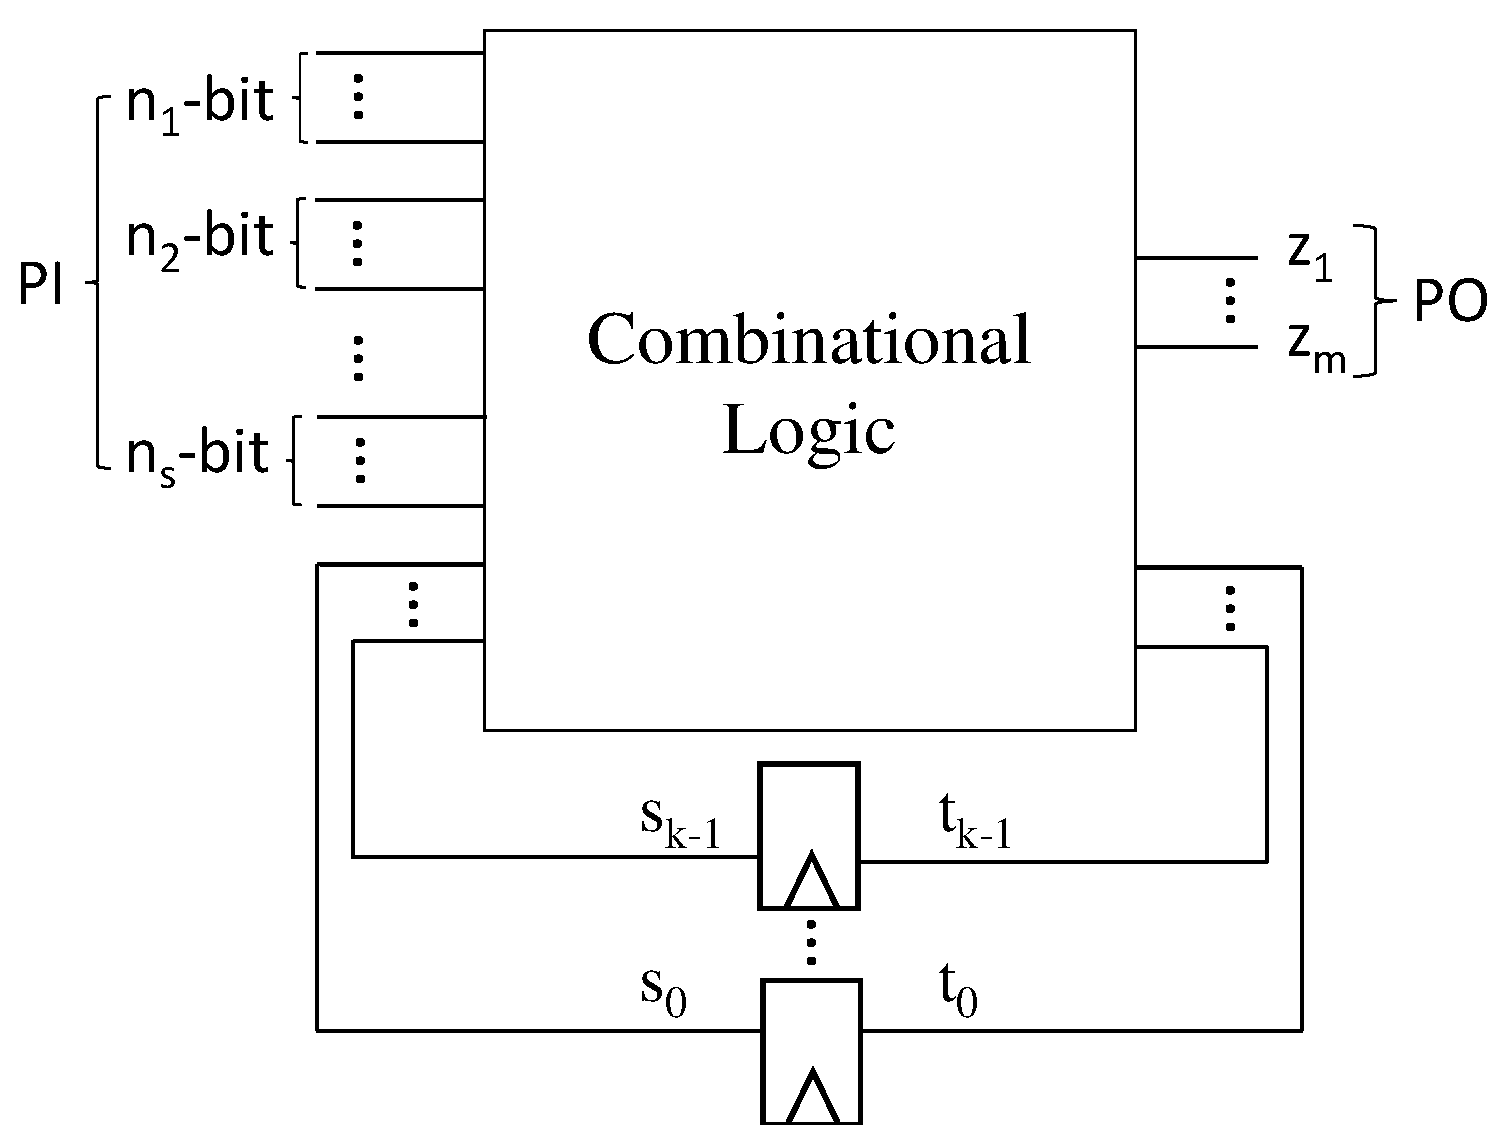
\includegraphics[width=\textwidth]{newfig/PI.pdf}
\caption{PI partition of a sequential circuit}
\label{fig:PI}}
\end{figure}

Assume we have $k$-bit datapath and $n$-bit PIs. In finite field, we need to carefully partition $n$ PIs
such that states of each partition can be covered by a univariate polynomial respectively.

\begin{Proposition}
Divide $n$-bit PIs into partitions $n_1,n_2,\dots, n_s$ where each $n_i|k$. Then let $n_1$-bit, $n_2$-bit, $\dots$, $n_s$-bit word-level variables
represent their evaluations in $\mathbb F_{2^k}$ as $\F_{2^{n_i}} \subset \Fkk$.
\end{Proposition}

Again, assume a partition $n_i~|~k$ and corresponding word-level variable is $P$. Then we can use polynomial
$P^{2^{n_i}}-P$ to represent all signals at free-end PIs, according to following theorem about {\bf composite
fields} \cite{ecc:software}:
\begin{Theorem}
\label{thm:composite}
Let $k = m\cdot n_i$, such that $\mathbb F_{2^k} = \mathbb F_{(2^{n_i})^m}$. Let $\alpha$ be primitive root of 
$\mathbb F_{2^k}$, $\beta$ be primitive root of the ground field $\mathbb F_{2^{n_i}}$. Then
$$\beta = \alpha^\omega,~~\text{where}~~\omega = \frac{2^k-1}{2^{n_i}-1}$$
\end{Theorem}
\begin{Example}
\label{ex:PI}
In a sequential circuit, PS/NS inputs/outputs are 4-bit signals, which means we will use $\mathbb F_{2^4}$
as working field. PIs are partitioned to 2-bit vectors, which means the ground field is $\mathbb F_{2^2}$.
In ground field we can represent all possible evaluations of this PI partition $\{p_0,p_1\}$ with
$$P^4+P,~~\text{where}~~P=p_0+p_1\cdot\beta$$
Using Theorem \ref{thm:composite} we get $\beta = \alpha^5$, so we can redefine word $P$ as element from $\mathbb F_{2^4}$:
$$P = p_0 + p_1\cdot\alpha^5$$
\end{Example}
Using this method we can efficiently partition large size PIs to small number of word-level PI variables.
One limitation of this approach is PIs cannot be partitioned when $k$ is prime.

\section{Implementation of Word-Level FSM Traversal Algorithm}
In this section, we describe the architecture of our tool which can perform word-level FSM traversal
on FSM benchmark circuits. Our tool consists of 3 functional components.
% First, the given circuit is synthesized to gate-level using state-of-art synthesizers.
First, the gate-level netlist of circuit is translated to polynomial form and variables are sorted in 
RATO. This part is implemented using a scripting language such as \emph{Perl}. If 
the given benchmark is a structural/behavior hybrid description, we perform pre-processing on it to get a synthesized netlist.
Secondly, the polynomial reduction is executed using our customized reduction engine, which is written in C++.
Finally, we utilize the symbolic computation engine \textsc{Singular} \cite{DGPS} to code Algorithm 
\ref{alg:refined} and execute the BFS traversal. The tool outputs a univariate polynomial 
for NS word $T$, denoting the set of reachable states from given initial state.

Figure \ref{fig:flowchart} illustrates the execution of reachability analysis approach
based on C++ and \textsc{Singular} implementation.

\begin{figure}[H]
\centering{
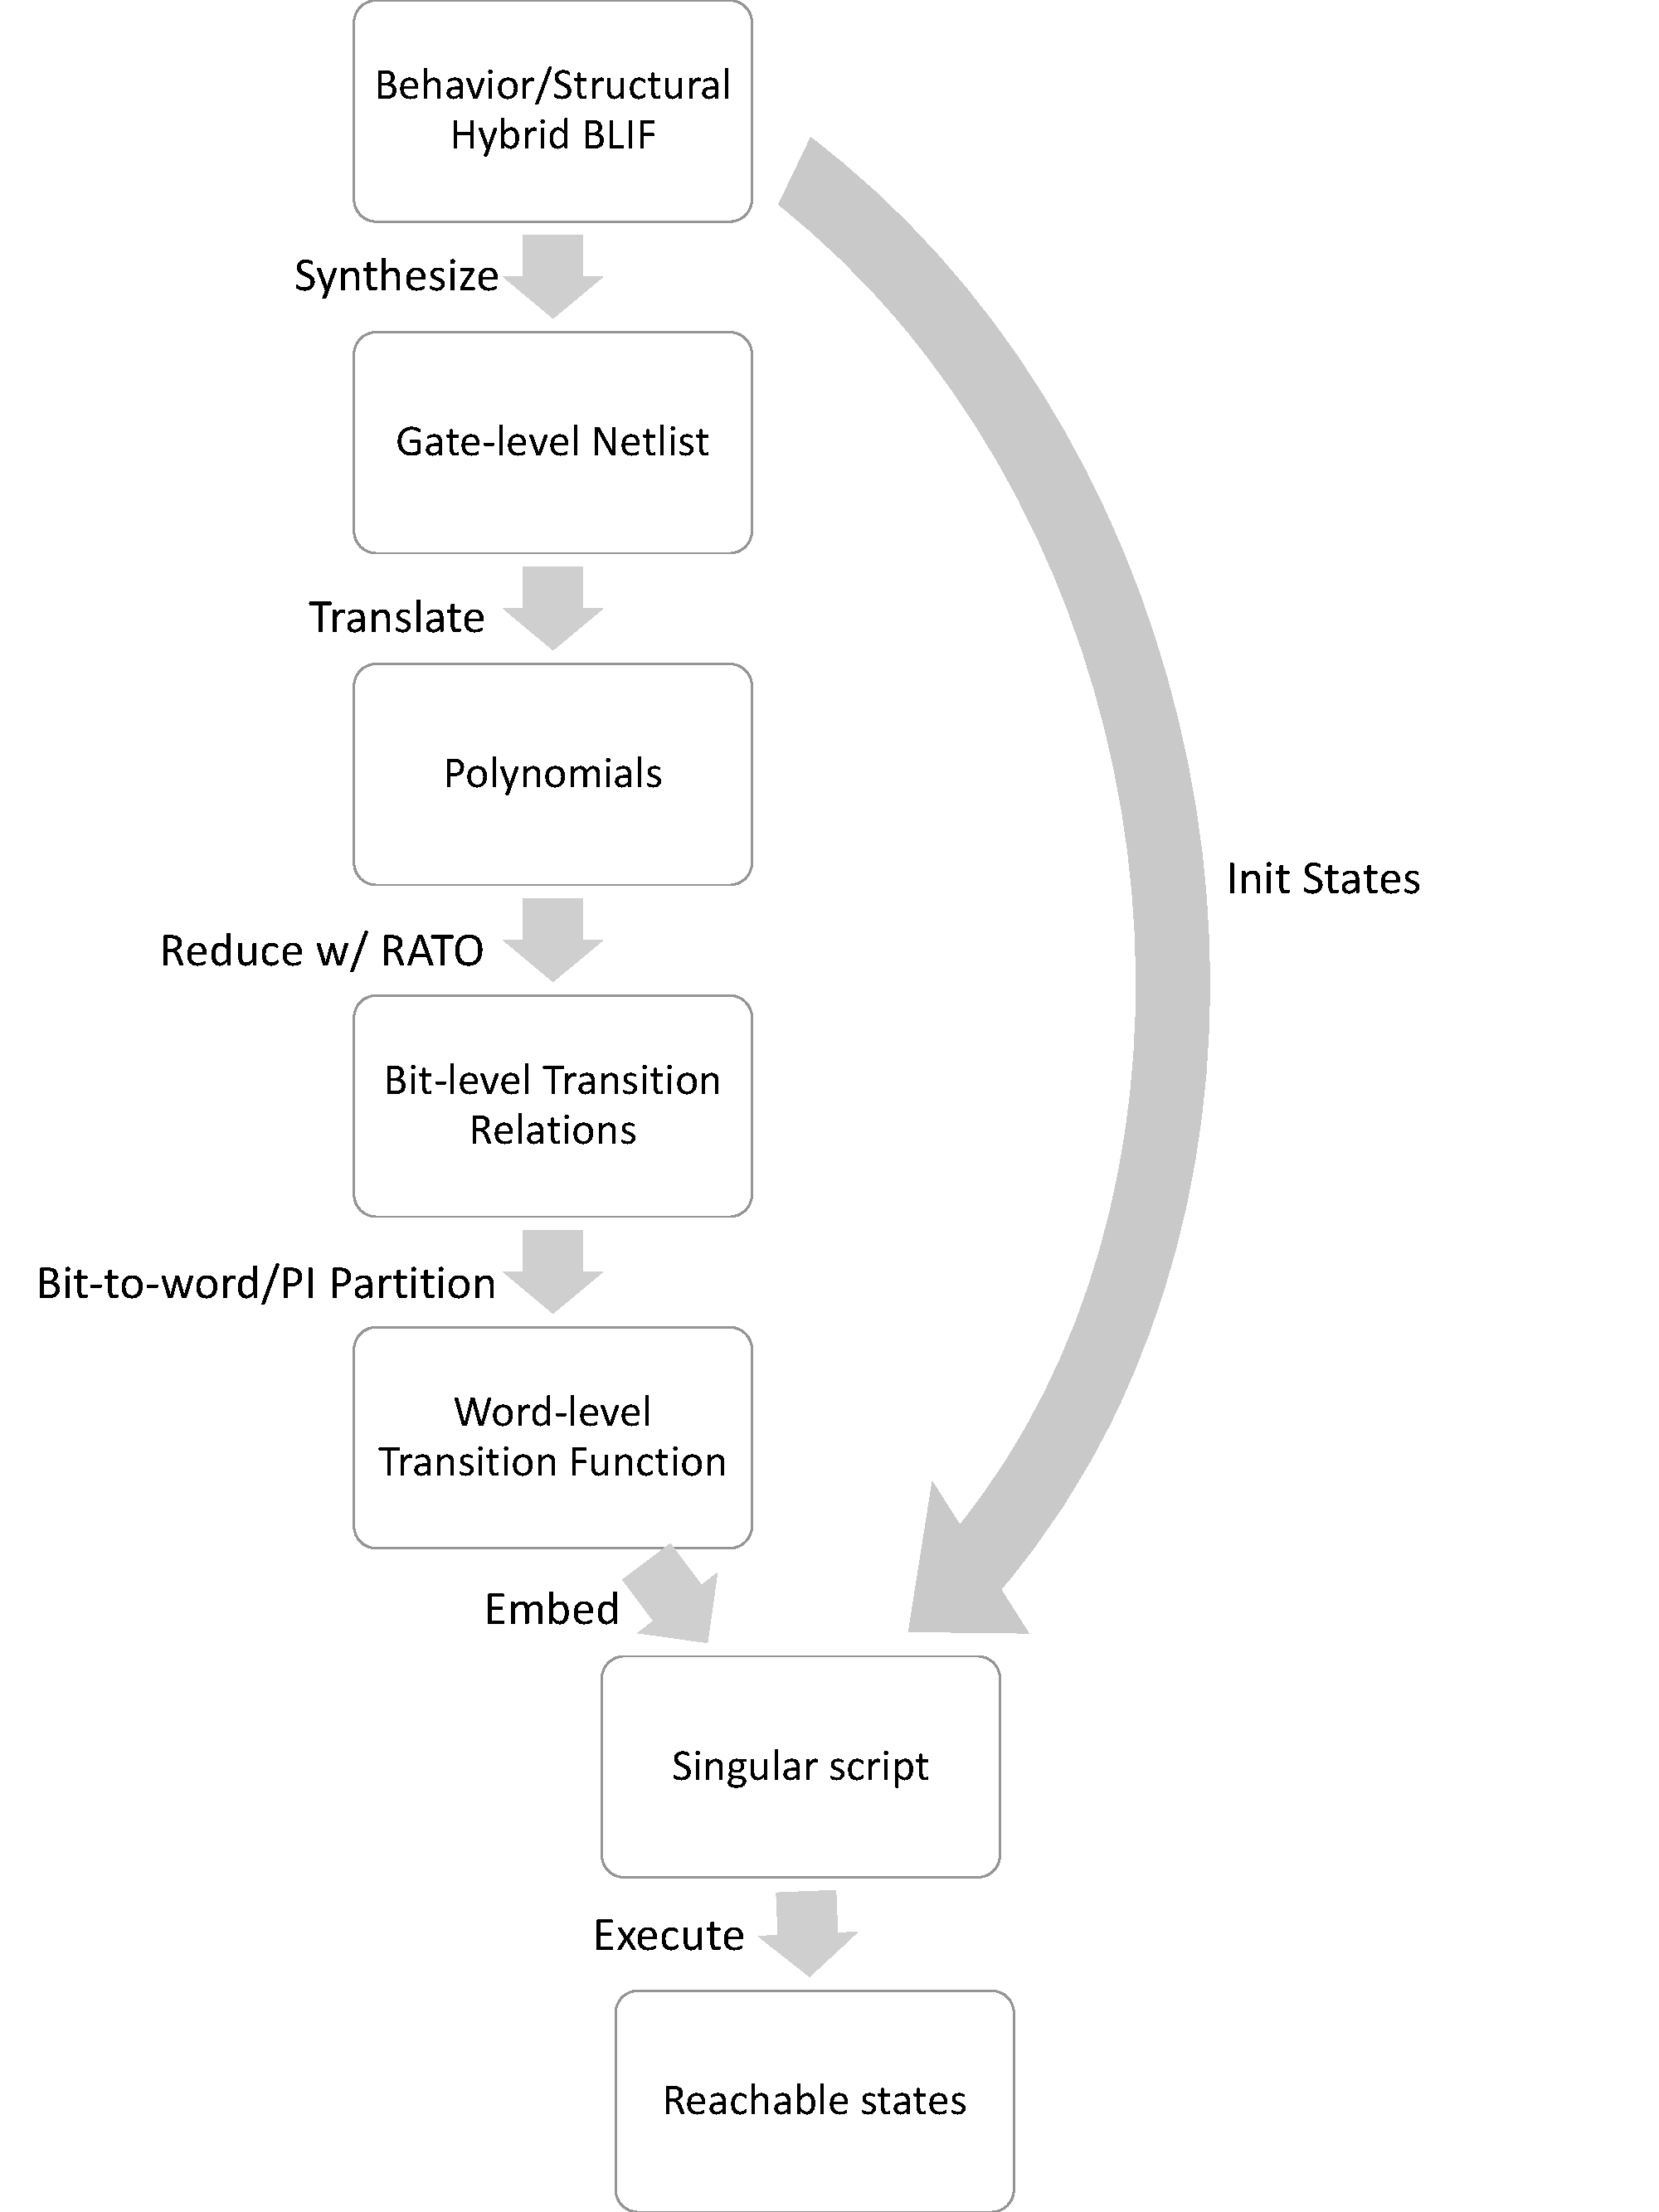
\includegraphics[width=\textwidth]{newfig/flowchart.pdf}
\caption{Execution process of word-level FSM traversal tool}
\label{fig:flowchart}}
\end{figure}

Usually FSM designs can be described in behavior/structural hybrid languages.
One of these languages is the Berkeley logic interchange format (BLIF) \cite{BLIF},
it allows state behavior representation and logic component representation.

\begin{Example}
In this example, we use benchmark FSM ``lion9" from MCNC benchmark library.
This benchmark circuit is given as state table based BLIF representation of a FSM.

% \begin{figure}[hbt]
% \centering{
% 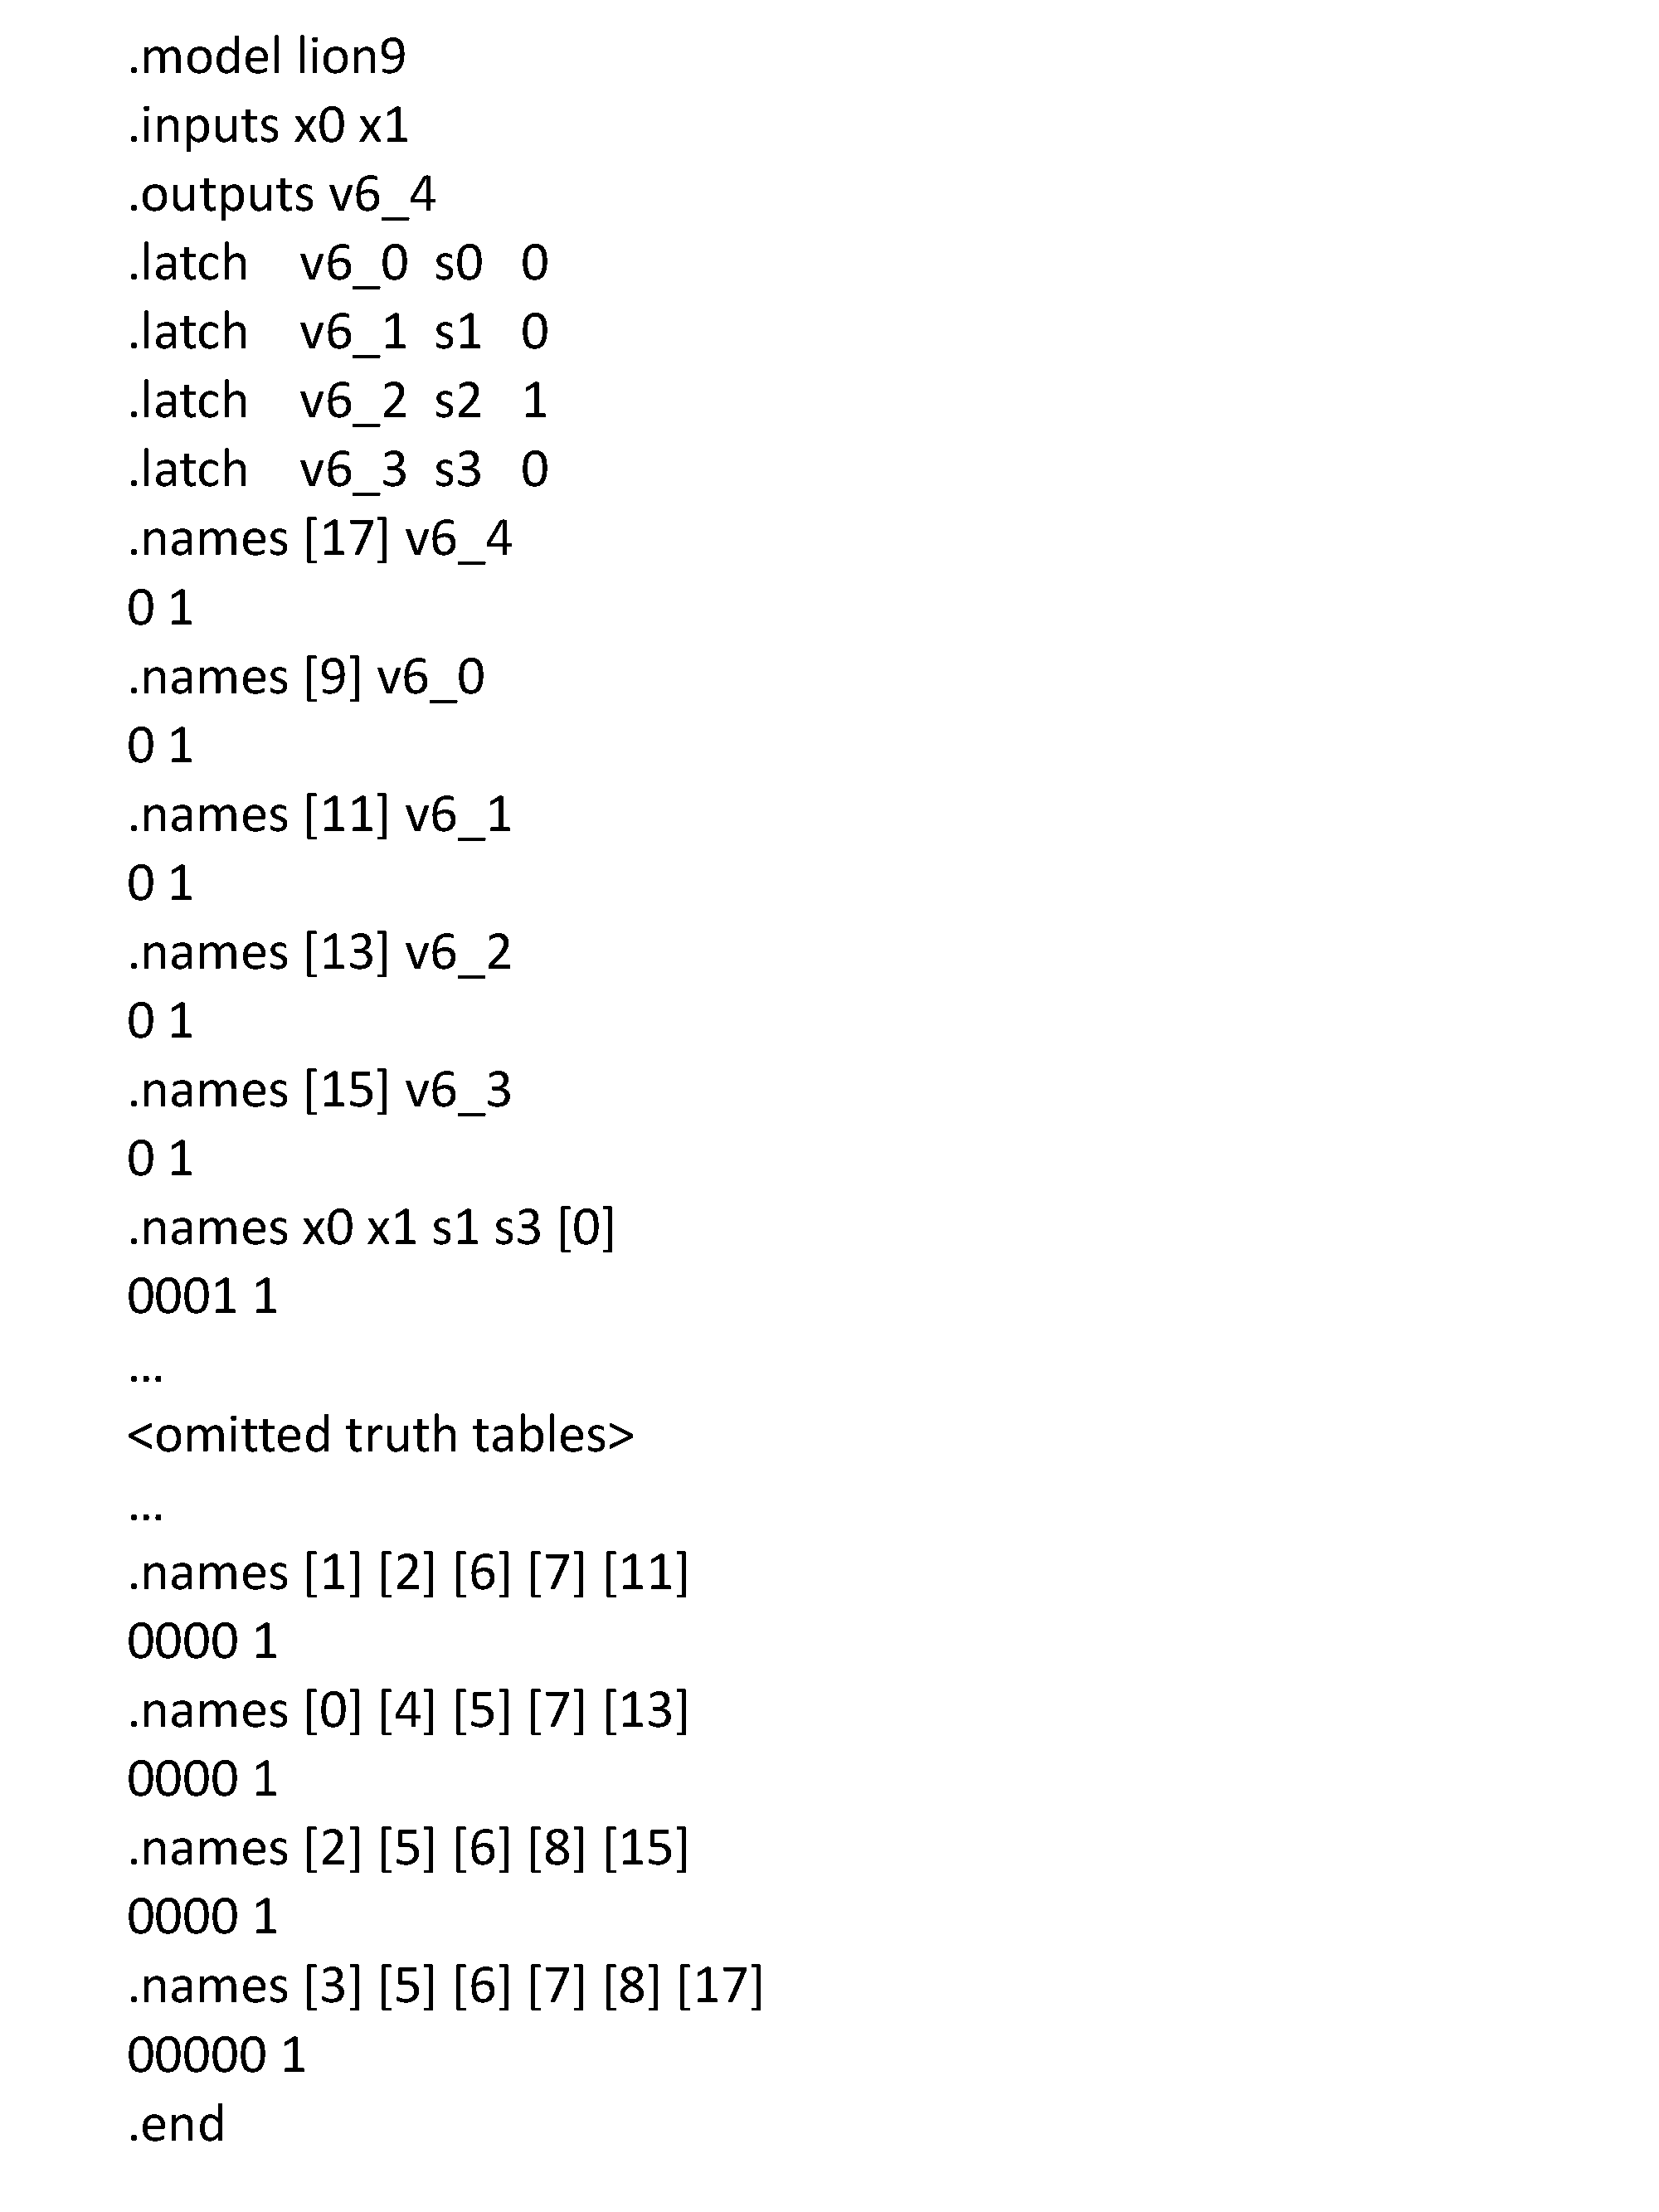
\includegraphics[width=\textwidth]{newfig/BLIF.pdf}
% \caption{Sample input BLIF file}
% \label{fig:BLIF}}
% \end{figure}

In order to compose the polynomial set in elimination ideal, we need to synthesize it to a 
gate-level netlist. Modern synthesizers including ABC \cite{brayton2010abc} and SIS \cite{SIS} 
can perform this task. In this example we use a synthesis library containing only 2-input 
AND, NAND, OR, NOR, XOR, XNOR gates as well as the inverter, the synthesized FSM is also given in 
BLIF format.

% \begin{figure}[hbt]
% \centering{
% 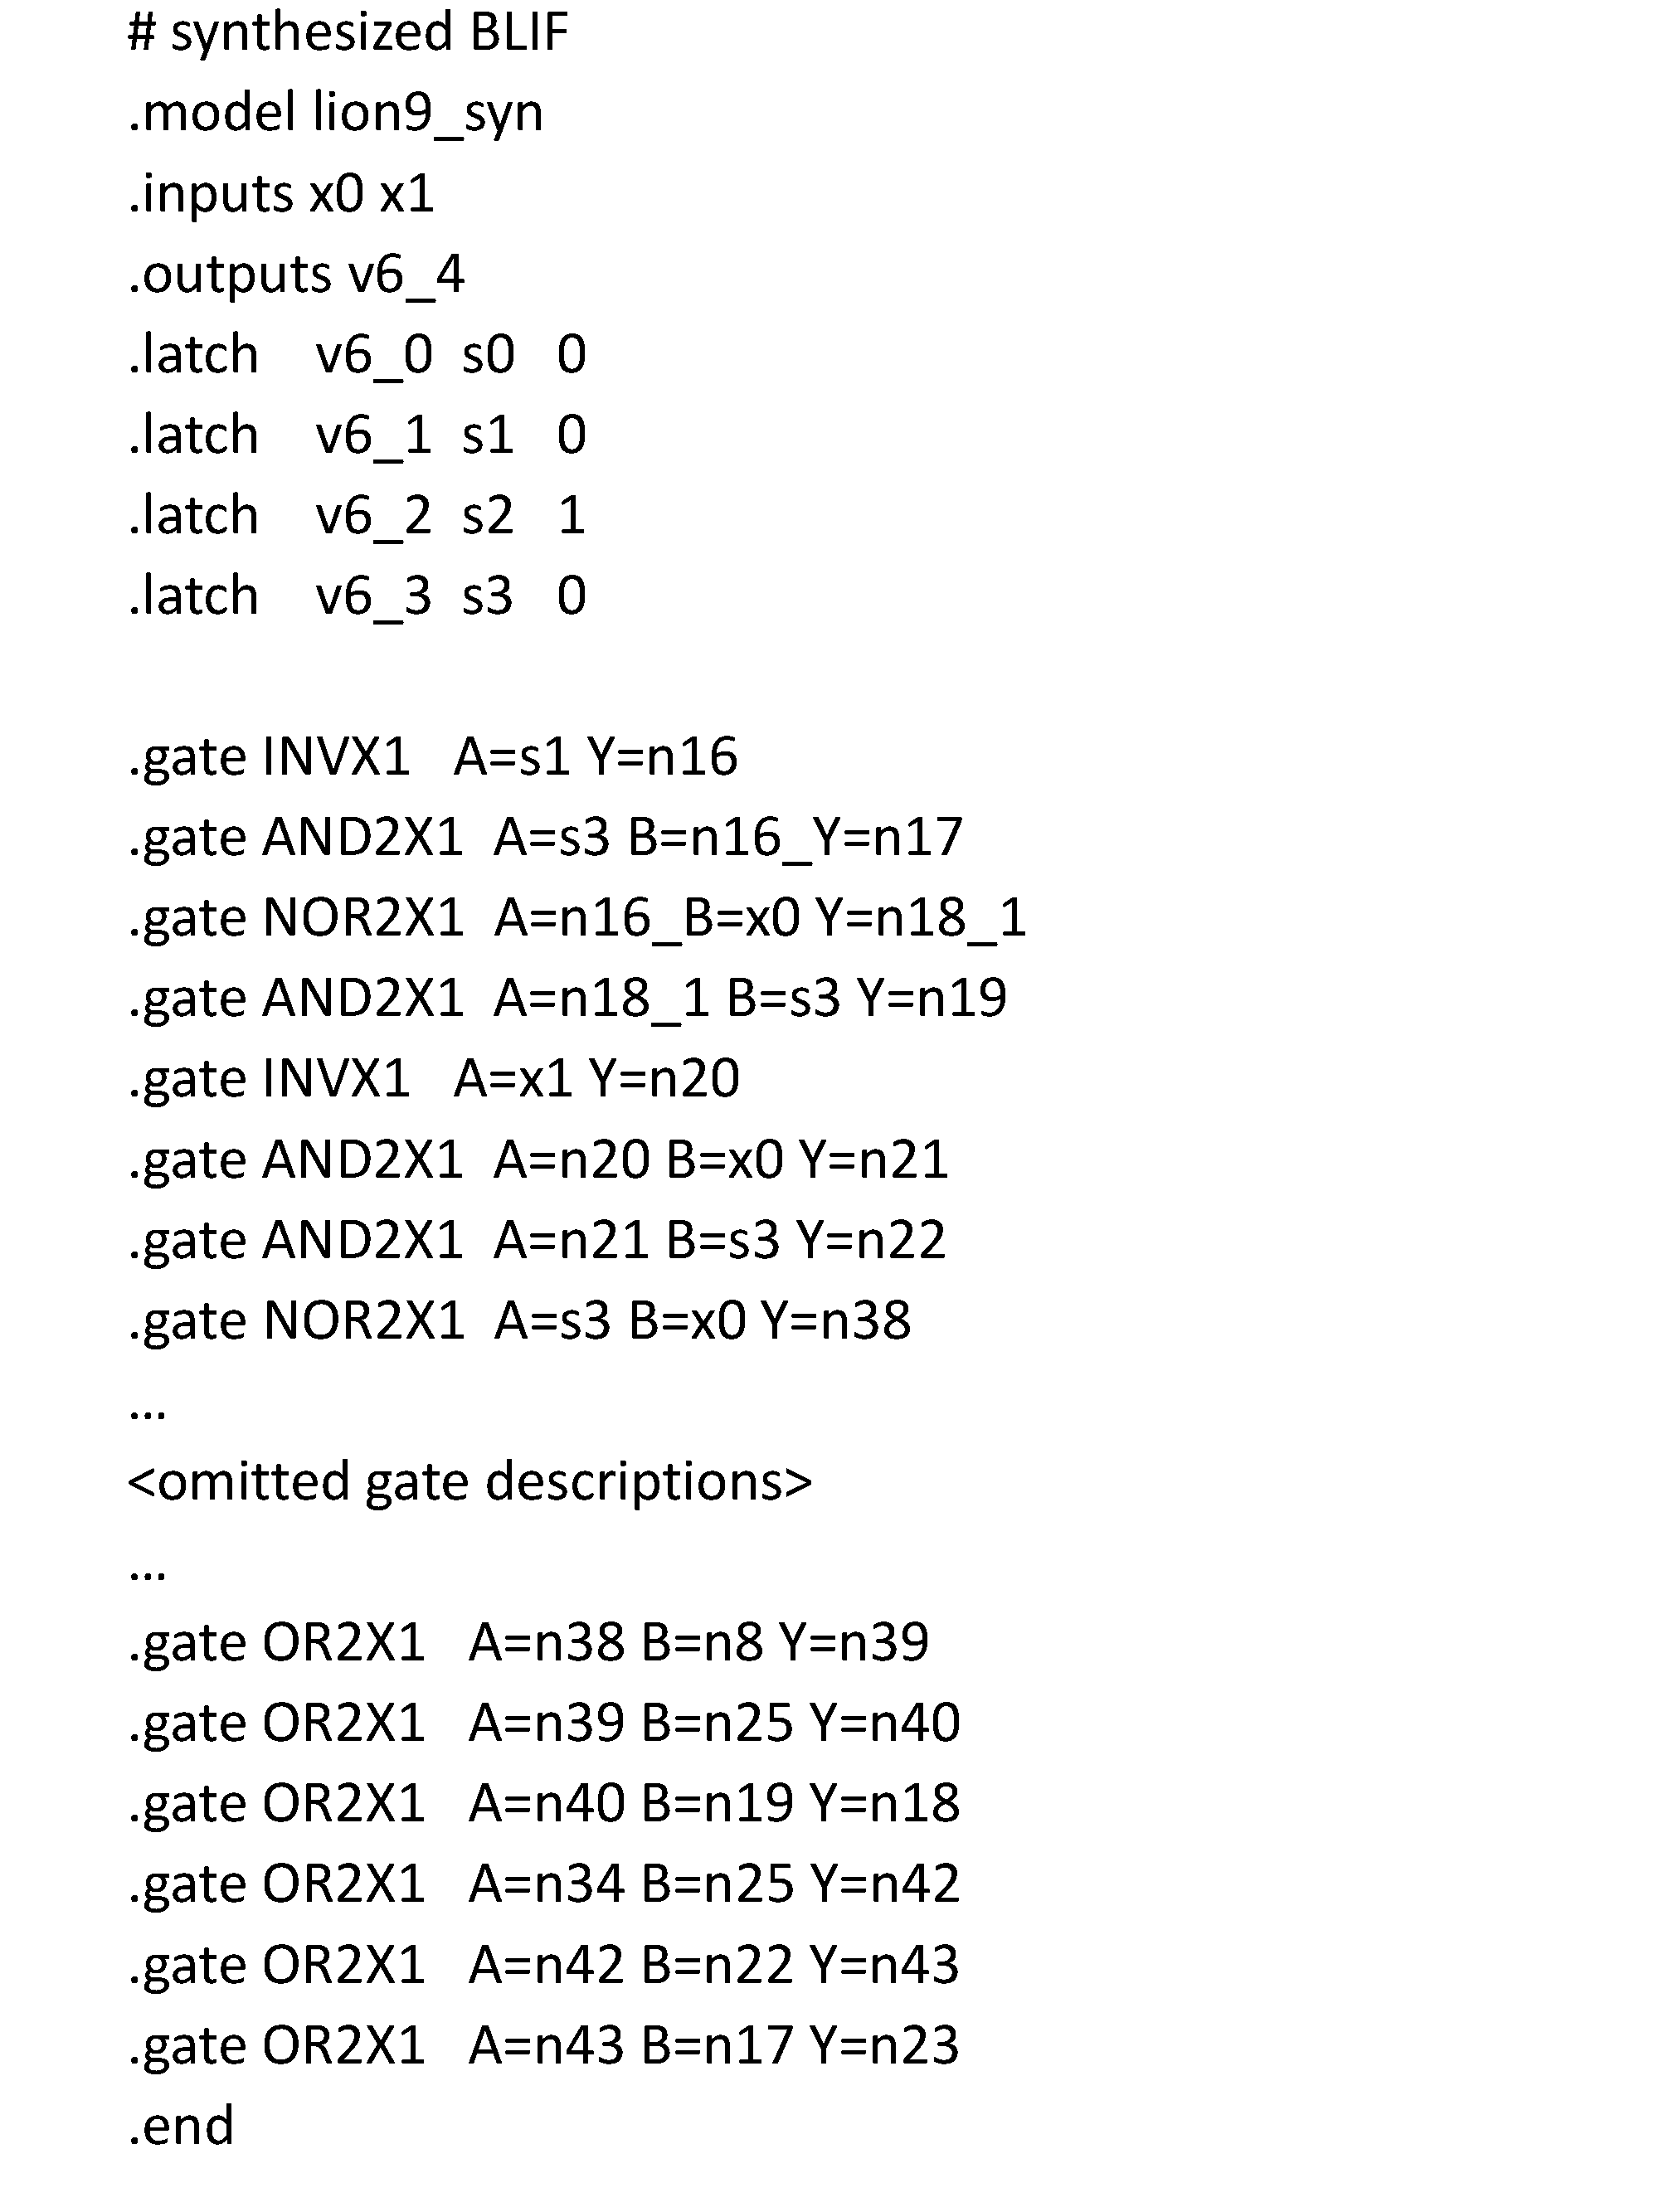
\includegraphics[width=\textwidth]{newfig/BLIF_syn.pdf}
% \caption{Synthesized BLIF file}
% \label{fig:BLIF_syn}}
% \end{figure}

Using our interpreter, the synthesized BLIF file is translated to a polynomial file customized for our 
polynomial reduction engine. 
The input file format includes all 
variables in RATO, along with the $Spoly$ that is need to be reduced, and polynomials in $J_{ckt}$.
% 
% \begin{figure}[hbt]
% \centering{
% 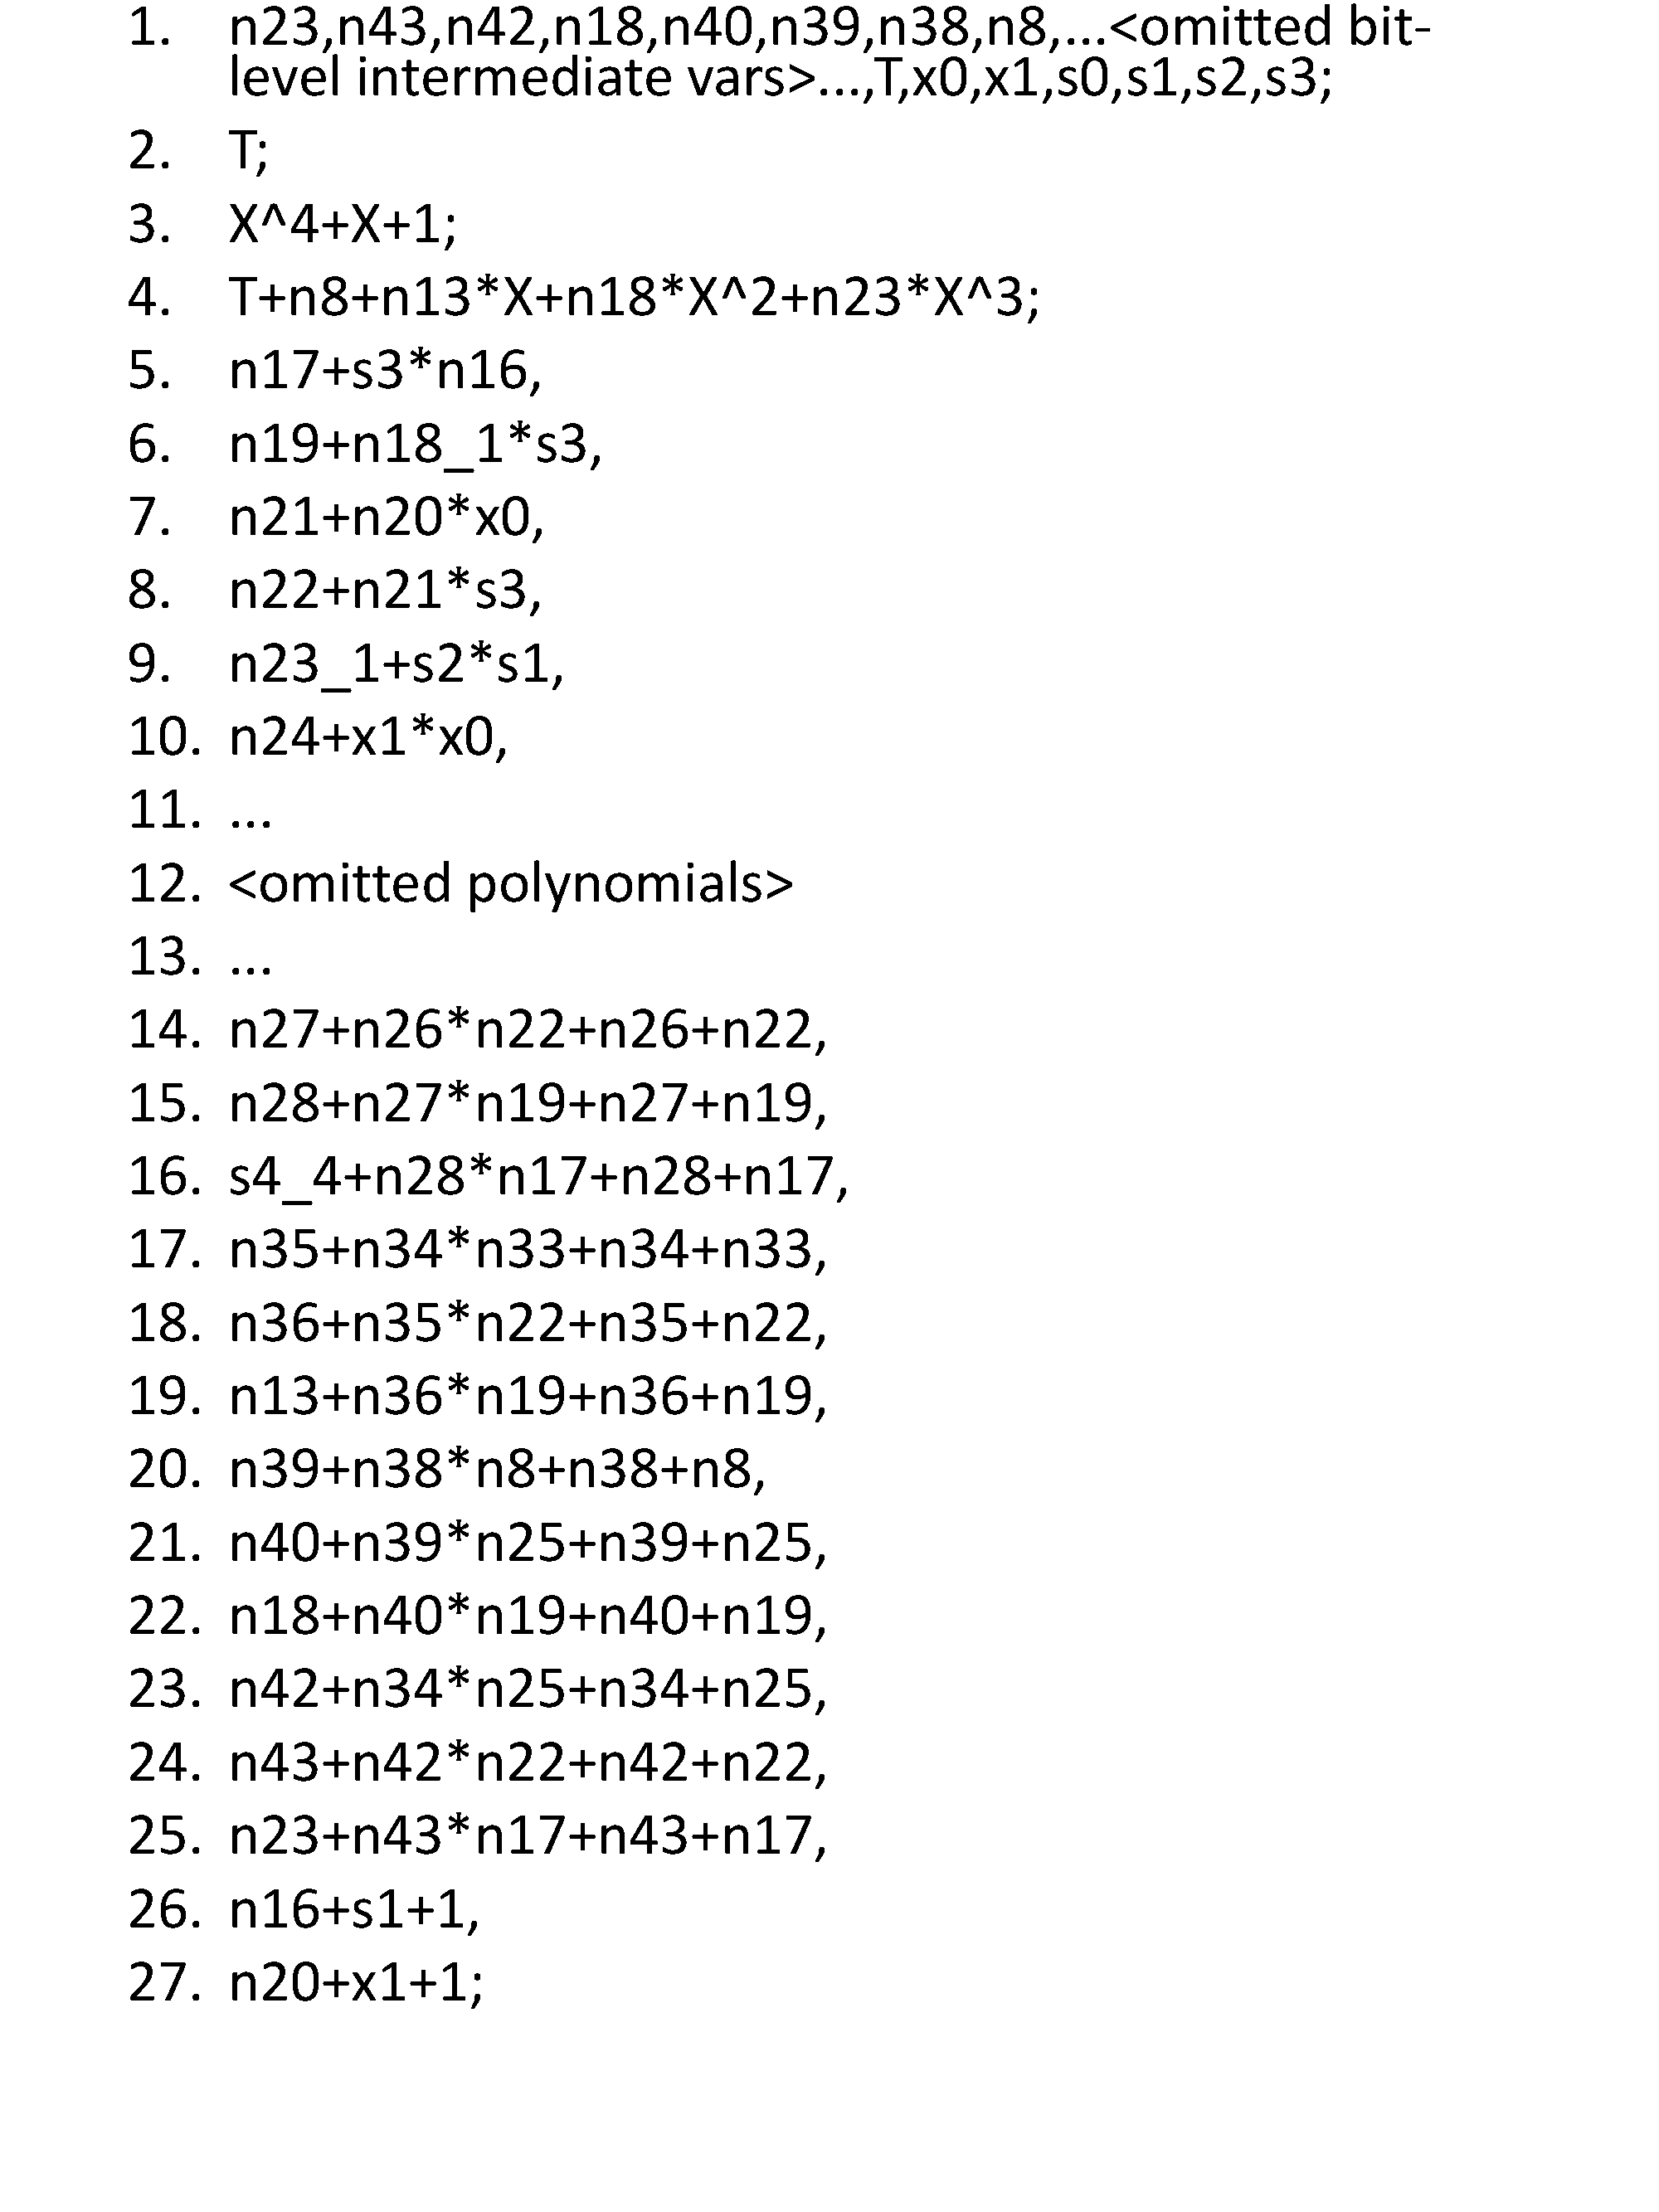
\includegraphics[width=\textwidth]{newfig/ALG.pdf}
% \caption{Polynomial file prepared for polynomial reduction engine}
% \label{fig:ALG}}
% \end{figure}

The result given by our reduction engine is in the form of the polynomial
$$T+\Func(s_0,\dots,s_{k-1},x_0,\dots,x_{n-1})$$ 
where $s_i$ and $x_j$ denote bit-level PS variables and PIs. Concretely in this example, the result is
\begin{align*}
T&+(\alpha^2+\alpha+1) x_0 x_1 s_1 s_3+(\alpha^3+\alpha) x_0 x_1 s_1+(\alpha+1) x_0 x_1 s_3 \\
&+(\alpha^3+1) x_0 s_1 s_3+(\alpha^3+\alpha) x_0 s_1 +(\alpha+1) x_0 s_3+(\alpha^2) x_0 \\
&+(\alpha^2+\alpha+1) x_1 s_1 s_3+(\alpha^3+\alpha) x_1 s_1+(\alpha^2+\alpha+1) x_1 s_3\\
&+(\alpha) x_1+(\alpha^3+1) s_1 s_3+(\alpha^3+\alpha) s_1+(\alpha^3+1) s_3+\alpha^2
\end{align*}
This is the transition function of this FSM. We utilized \textsc{Singular} to integrate both 
bit-to-word substitution and the traversal algorithm. In Figure \ref{fig:SING}, ``tran" is the transition
function we just obtained. ``init\_S" is the initial state, note it equals to ``0100" register 
reset values preloaded in the BLIF file. Moreover, 2 bits PIs $x_0,x_1$ are combined to a word-level 
PI variable $P$ using our conclusion in Example \ref{ex:PI}: ``def\_X" is the definition of 2-bit 
word, and ``red\_X" denotes the vanishing polynomial for word $P$.


After the script is executed, the traversal finishes after 4 
transition iterations, which denotes BFS depth equals to 4. The final reachable states 
is a degree-9 polynomial in $T$, indicating final reachable states set contains 9 states.
And state encodings can be obtained by solving this polynomial equation.

\begin{figure}[H]
\centering{
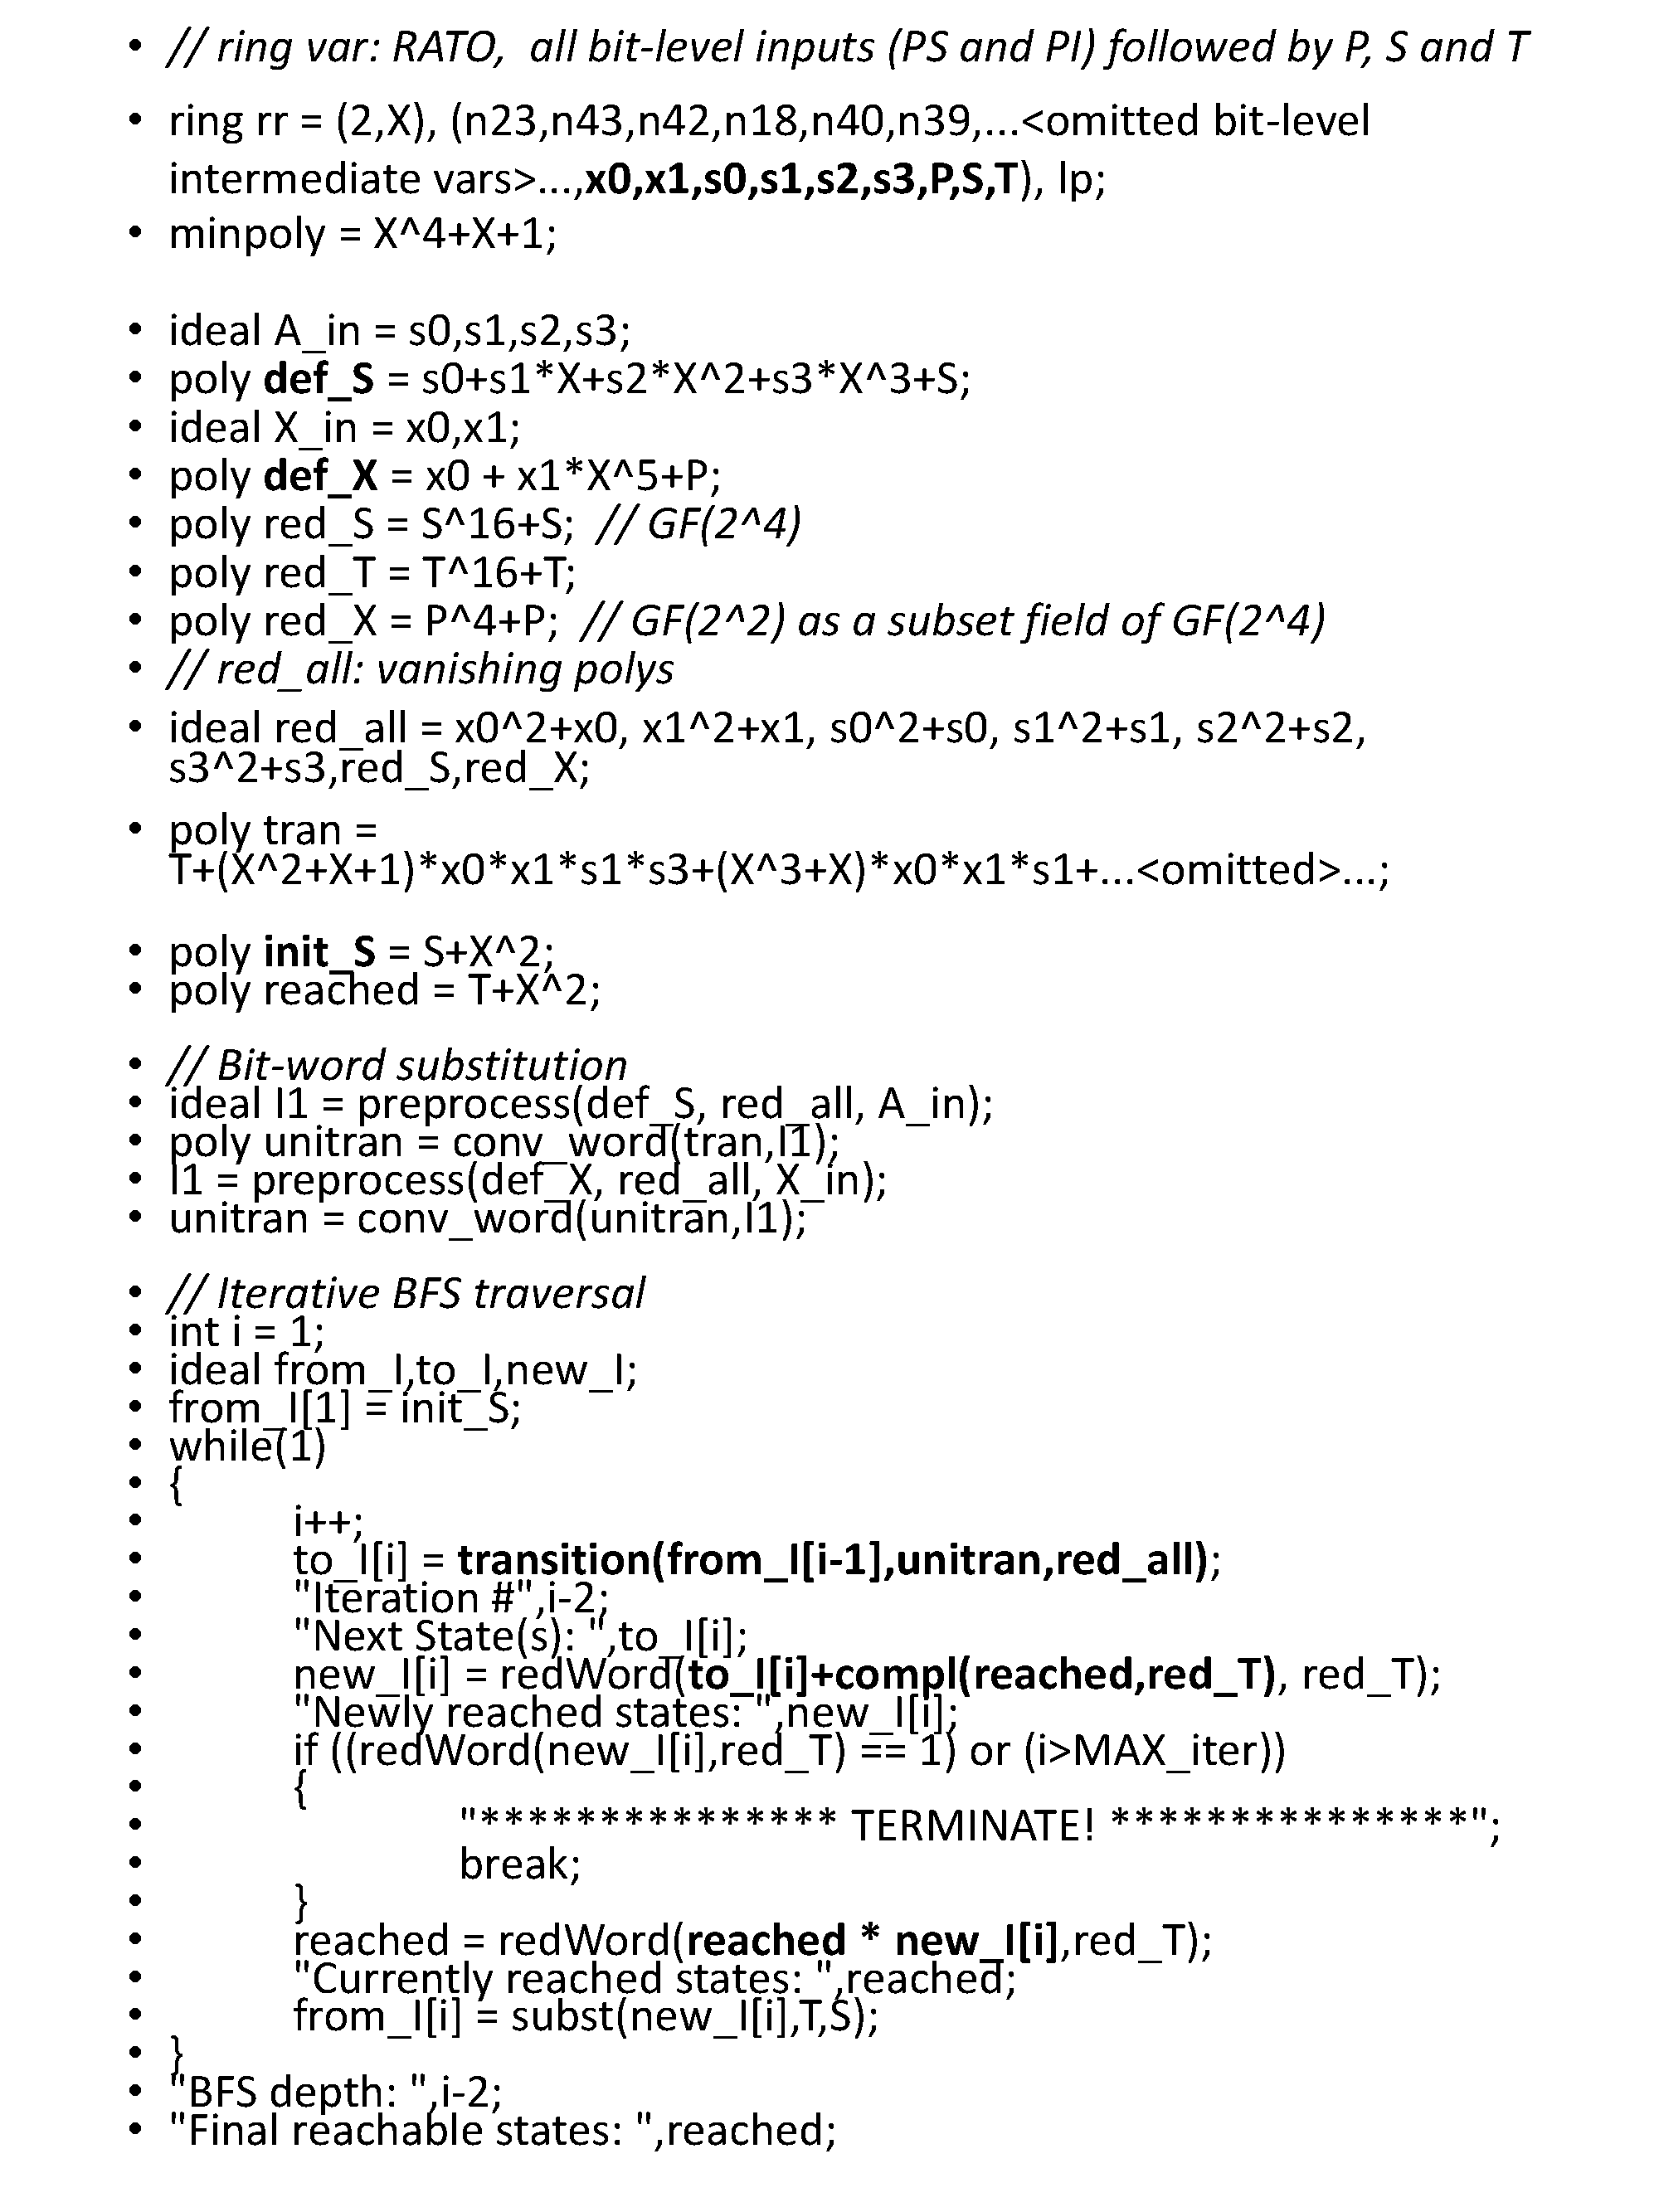
\includegraphics[width=\textwidth]{newfig/SING.pdf}
\caption{Singular script for executing bit-to-word substitution and traversal loop}
\label{fig:SING}}
\end{figure}


\begin{figure}[H]
\centering{
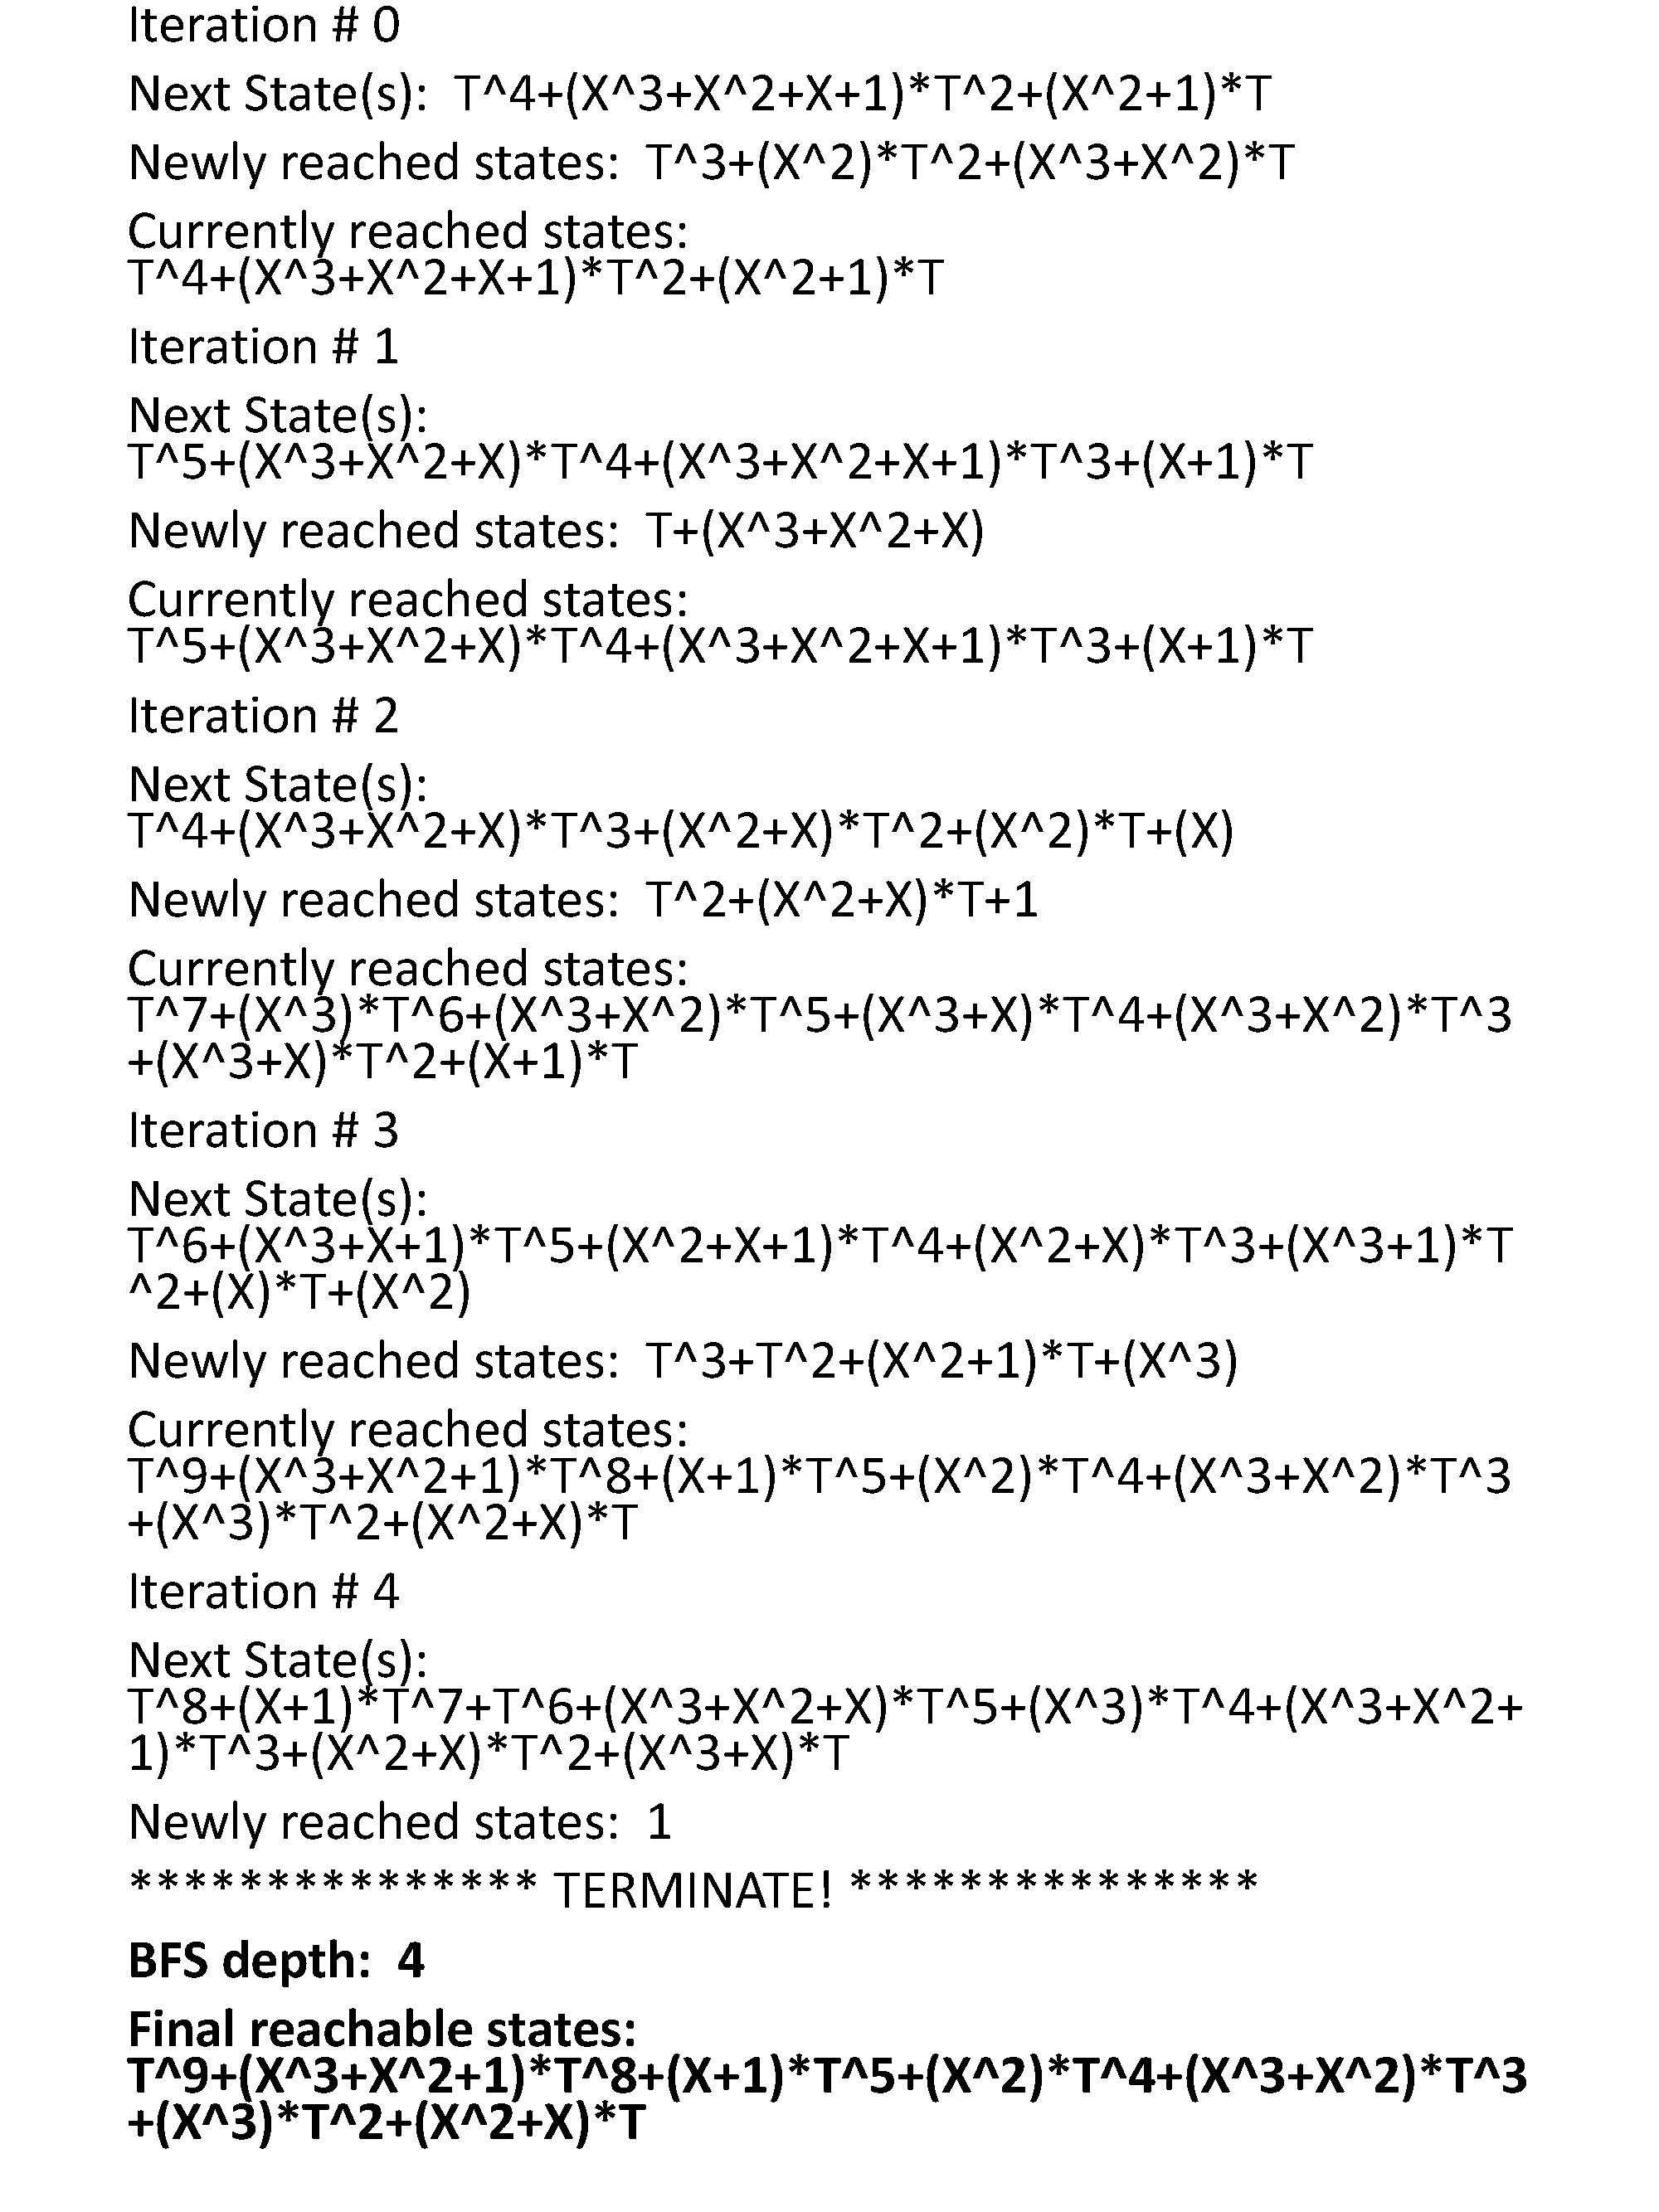
\includegraphics[width=\textwidth]{newfig/Recha_result.pdf}
\caption{The output given by our traversal tool}
\label{fig:Recha_result}}
\end{figure}

\end{Example}

\section{Experiment Results}
\label{sec:exp_reacha}
We have implemented our traversal algorithm in 3 parts:
the first part implements polynomial reductions (division) of the
Gr\"obner basis computations, under the term order derived from the
circuit as Line 2 in Algorithm \ref{alg:refined}. This is implemented 
with our customized data structure in
C++. The second part implements the bit-level to word-level
abstraction to attain transition functions at the word-level 
%$T+\mathcal{F}(S,PIs)$ 
using the \textsc{Singular} symbolic
algebra computation system [v. 3-1-6] \cite{DGPS}, as Line 3 in 
Algorithm \ref{alg:refined}; and the third part
executes the reachability checking iterations using 
\textsc{Singular} as well. With our
tool implementation, we have performed experiments to analyze reachability
of several FSMs. Our experiments run on a desktop with
3.5GHz Intel $\text{Core}^\text{TM}$ i7-4770K Quad-core CPU, 32 GB RAM and
64-bit Ubuntu Linux OS. The experiments are shown in Table \ref{tab:recha_result}. 

There are 2 bottlenecks which restricts the performance of our tool:
one bottleneck is that the polynomial reduction engine is slow when the number of
gates (especially OR gates) is large; the other one is the high computational complexity
of Gr\"obner basis engine in general. Therefore, we pick 10 FSM
benchmarks of reasonable size for testing our tool. Among them ``b01,
b02, b06" come from ITC'99 benchmarks, %\cite{ITC99}, 
``s27, s208, s386" are from  ISCAS'89 benchmarks %\cite{yang1991logic}
 and ``bbara, beecount, dk14, donfile" are from MCNC benchmarks. %\cite{yang1991logic}.
ISCAS benchmarks are given in {\it bench} format so we can directly read gate information,
where ITC/MCNC FSMs are given in unsynthesized {\it BLIF} format so we first turn them
into gate-level netlists using AIG based synthesizer ABC. % \cite{brayton2010abc}.
Since the number of primary inputs $(m)$ is relatively small, in our experiments we partition
primary inputs as $m$ single bit-level variables. To verify the
correctness of our techniques and implementations, we compare the
number of reachable states obtained from our tool against the results
obtained from the VIS tool \cite{brayton1996vis}. 

\begin{table}[H]
\centering
\caption{Results of running benchmarks using our tool. 
\small{Parts I to III denote the time taken by polynomial divisions,
  bit-level to word-level abstraction and iterative reachability
  convergence checking part of our approach, respectively.}}
{\small 
\begin{tabular}{|c||c|c|c|c|c|c|c|c|c|}
\hline
\multirow{3}{*}{\centering Benchmark} 
& \multirow{3}{0.9cm}{\centering \# Gates} 
& \multirow{3}{1.1cm}{\centering \# Latches} 
& \multirow{3}{*}{\centering \# PIs}
 & \multirow{3}{0.9cm}{\centering \# States}
 & \multirow{3}{1.3cm}{\centering \# iterations}
 & \multicolumn{3}{c|}{\multirow{2}{2.0cm}{\centering Runtime (sec)}}
 & \multirow{3}{1.8cm}{\centering Runtime of VIS (sec)} \\
  & & & & & &\multicolumn{3}{c|}{}& \\
  \cline{7-9}
    & & & & & & I & II & III & \\
\hline
\hline
b01 & 39  & 5  & 2 & 18  & 5  & $<0.01$ & 0.01 & 0.02 & $<0.01$\\
b02 & 24  & 4  & 1 & 8 & 5 & $<0.01$  & 0.01 & $<0.01$ & $<0.01$ \\
b06 & 49  & 9  & 2 & 13 & 4 & $<0.01$ & 0.07 & 5.0 & $<0.01$ \\
s27 & 10 & 3 & 4 & 6 & 2 & $<0.01$ & 0.01 & 0.02  & $<0.01$  \\
s208 & 61 & 8 & 11 & 16 & 16 & $<0.01$ & 0.32 & 2.4 & $<0.01$ \\
s386 & 118 & 6 & 13 & 13  & 3 & 1.0 & 7.6 & 8.2  & $<0.01$ \\
bbara & 82 & 4 & 4 & 10 & 6 & 0.04 & 0.01 & 0.04  & $<0.01$ \\
beecount & 48  & 3  & 3 & 7  & 3  &$<0.01$ & 0.01 & 0.01 & $<0.01$ \\
dk14 & 120  & 3  & 3 & 7  & 2  & 45 & $<0.01$ & 0.08 & $<0.01$\\
donfile & 205  & 5  & 2 & 24 & 3  & 12316 & 0.02 & 1.7  & $<0.01$\\
\hline
\end{tabular}
}
\label{tab:recha_result}  
\end{table} 

In Table \ref{tab:recha_result}, \# States denotes the final reachable states
starting from given reset state, which given by our tool is the same with
the return value of {\it compute\_reach} in VIS. Meanwhile, from observation
of the experiment run-times, we find the reduction runtime increases
as the number of gates grows. Also, iterative reachability convergence
check's runtime reflects both the size of present state/next state
words ($k$) and the number of final reached states, which corresponds
to the degree of polynomial {\it reached} in Algorithm \ref{alg:univa}. 
Although the efficiency of our initial implementation fails to compete
with the BDD based FSM analyzer VIS, the experiment
demonstrates the power of abstraction of algebraic geometry techniques
for reachability analysis applications. 
% Currently, we are investigating techniques that
% can help us overcome the complexity of the GB computation with elimination
% orders and speed-up our approach. 

%\vspace{-0.1in}

\section{Concluding Remarks}
This chapter has presented a new approach to perform reachability
analysis of finite state machines at the word-level. This is achieved
by modeling the transition relations and sets of states by way of
polynomials over finite fields $\Fkk$, where $k$ represents the size
of the state register bits. Subsequently using the concepts of
elimination ideals, Gr\"obner bases, and quotients of ideals, we show
that the set of reachable states can be encoded, canonically, as the
variety of a univariate polynomial. This polynomial is computed using
the Gr\"obner basis algorithm {\it w.r.t.} an elimination term
order. Experiments are conducted with a few FSMs that validate the
concept of word-level FSM traversal using algebraic geometry. 
